% Options for packages loaded elsewhere
\PassOptionsToPackage{unicode}{hyperref}
\PassOptionsToPackage{hyphens}{url}
\PassOptionsToPackage{dvipsnames,svgnames*,x11names*}{xcolor}
%
\documentclass[
]{article}
\usepackage{lmodern}
\usepackage{amsmath}
\usepackage{ifxetex,ifluatex}
\ifnum 0\ifxetex 1\fi\ifluatex 1\fi=0 % if pdftex
  \usepackage[T1]{fontenc}
  \usepackage[utf8]{inputenc}
  \usepackage{textcomp} % provide euro and other symbols
  \usepackage{amssymb}
\else % if luatex or xetex
  \usepackage{unicode-math}
  \defaultfontfeatures{Scale=MatchLowercase}
  \defaultfontfeatures[\rmfamily]{Ligatures=TeX,Scale=1}
\fi
% Use upquote if available, for straight quotes in verbatim environments
\IfFileExists{upquote.sty}{\usepackage{upquote}}{}
\IfFileExists{microtype.sty}{% use microtype if available
  \usepackage[]{microtype}
  \UseMicrotypeSet[protrusion]{basicmath} % disable protrusion for tt fonts
}{}
\makeatletter
\@ifundefined{KOMAClassName}{% if non-KOMA class
  \IfFileExists{parskip.sty}{%
    \usepackage{parskip}
  }{% else
    \setlength{\parindent}{0pt}
    \setlength{\parskip}{6pt plus 2pt minus 1pt}}
}{% if KOMA class
  \KOMAoptions{parskip=half}}
\makeatother
\usepackage{xcolor}
\IfFileExists{xurl.sty}{\usepackage{xurl}}{} % add URL line breaks if available
\IfFileExists{bookmark.sty}{\usepackage{bookmark}}{\usepackage{hyperref}}
\hypersetup{
  pdftitle={Approche méthodologique pour évaluer la faisabilité du recyclage des polymères dans un contexte de fabrication additive open-source},
  colorlinks=true,
  linkcolor=blue,
  filecolor=Maroon,
  citecolor=Blue,
  urlcolor=Blue,
  pdfcreator={LaTeX via pandoc}}
\urlstyle{same} % disable monospaced font for URLs
\usepackage[margin=1in]{geometry}
\usepackage{graphicx}
\makeatletter
\def\maxwidth{\ifdim\Gin@nat@width>\linewidth\linewidth\else\Gin@nat@width\fi}
\def\maxheight{\ifdim\Gin@nat@height>\textheight\textheight\else\Gin@nat@height\fi}
\makeatother
% Scale images if necessary, so that they will not overflow the page
% margins by default, and it is still possible to overwrite the defaults
% using explicit options in \includegraphics[width, height, ...]{}
\setkeys{Gin}{width=\maxwidth,height=\maxheight,keepaspectratio}
% Set default figure placement to htbp
\makeatletter
\def\fps@figure{htbp}
\makeatother
\setlength{\emergencystretch}{3em} % prevent overfull lines
\providecommand{\tightlist}{%
  \setlength{\itemsep}{0pt}\setlength{\parskip}{0pt}}
\setcounter{secnumdepth}{-\maxdimen} % remove section numbering
\usepackage{multirow}
\usepackage{multicol}
\usepackage{colortbl}
\usepackage{hhline}
\usepackage{longtable}
\usepackage{array}
\usepackage{hyperref}
\ifluatex
  \usepackage{selnolig}  % disable illegal ligatures
\fi
\newlength{\cslhangindent}
\setlength{\cslhangindent}{1.5em}
\newlength{\csllabelwidth}
\setlength{\csllabelwidth}{3em}
\newenvironment{CSLReferences}[2] % #1 hanging-ident, #2 entry spacing
 {% don't indent paragraphs
  \setlength{\parindent}{0pt}
  % turn on hanging indent if param 1 is 1
  \ifodd #1 \everypar{\setlength{\hangindent}{\cslhangindent}}\ignorespaces\fi
  % set entry spacing
  \ifnum #2 > 0
  \setlength{\parskip}{#2\baselineskip}
  \fi
 }%
 {}
\usepackage{calc}
\newcommand{\CSLBlock}[1]{#1\hfill\break}
\newcommand{\CSLLeftMargin}[1]{\parbox[t]{\csllabelwidth}{#1}}
\newcommand{\CSLRightInline}[1]{\parbox[t]{\linewidth - \csllabelwidth}{#1}\break}
\newcommand{\CSLIndent}[1]{\hspace{\cslhangindent}#1}

\title{Approche méthodologique pour évaluer la faisabilité du recyclage
des polymères dans un contexte de fabrication additive open-source}
\author{}
\date{\vspace{-2.5em}}

\begin{document}
\maketitle

\hypertarget{ruxe9sumuxe9}{%
\section*{Résumé}\label{ruxe9sumuxe9}}
\addcontentsline{toc}{section}{Résumé}

Depuis de début du XXI siècle, nous avons assisté à la démocratisation
de l'impression 3D, en même temps que l'émergence du mouvement « Open
Source Hardware ». La conjonction de ces deux phénomènes a ouvert des
opportunités très significatives pour la conception dans l'industrie
manufacturière traditionnelle, mais aussi pour des nouvelles activités
telles que le recyclage des matières thermoplastiques. Dans ce chapitre
nous proposons une méthodologie générale permettant le recyclage de
polymères thermoplastiques dans le contexte open-source. La méthodologie
développée a été utilisée dans le cadre du recyclage de l'acide
polylactique (PLA). Nous montrons le niveau de dégradation de la matière
à travers l'ensemble du procédé grâce à la caractérisation des
propriétés mécaniques et physico-chimiques, et concluons qu'il est
possible de recycler le PLA pour l'impression 3D. Enfin, nous étudierons
les implications pour la diffusion de ce type de recyclage, et proposons
en perspective d'étudier le recyclage en circuit court d'autres
polymères thermoplastiques.

\textbf{Mot clés :} Recyclage des Polymères, Fabrication Additive,
Open-Source, Impression 3D, Acide Polylactique (PLA), RepRap.

\hypertarget{introduction}{%
\section{Introduction}\label{introduction}}

En ce début de \(XXI^{\grave{e}me}\) siècle, considérer qu'aujourd'hui
encore, seul la technique transformerait la société toute entière, est
clairement une hérésie. Certes, les révolutions techniques sont là:
explosion de l'internet, interconnexion et échanges entre personnes
(peer to peer), apparition de nouvelles formes d'énergie, de nouveaux
procédés de production, de nouveaux matériaux etc... mais l'homme n'est
plus un simple consommateur Keynésien sensible uniquement au prix et aux
incitations de l'état. Il souhaite désormais, être acteur et participer
à l'utilisation des nouvelles technologies mais de manière raisonnée et
en intégrant les grands enjeux sociétaux tels que le partage et la
sauvegarde des ressources et matières premières.

Dans le cadre de nos travaux nous présentons comment une révolution
technologique telle que la fabrication additive (FA) open source peut se
développer tout en intégrant les défis sociétaux actuels et plus
particulièrement les enjeux environnementaux. En effet cette dernière,
aussi connue comme \emph{impression 3D open-source (OS)} est l'une des
technologies identifiées comme ayant un fort potentiel d'impact sur les
systèmes de production, mais aussi plus largement, sur notre style de
vie dans les années à venir. Sa principale particularité par rapport à
la FA classique est le caractère collaboratif de l'open source qui
permet des évolutions rapides et créatives, et ceci à moindre coût. Dans
le cadre de ces travaux, nous préconiserons dans un premier temps ce
qu'est la FA au sens large et nous proposerons un état de l'art des
études menées sur le recyclage dans le contexte de la FA.

Enfin, nous nous intéresserons au potentiel de recyclage de polymères
dédiés à la FA open-source et nous proposerons une méthodologie
permettant la caractérisation de la dégradation physique de la matière
recyclée tout au long de la chaîne de recyclage et d'impression. Les
résultats de l'application de la méthodologie proposée au cas
particulier de l'acide polylactide (PLA), une matière largement utilisé
dans l'impression 3D, seront présentées comme preuve du concept. Pour
finir nous concluerons et rappellerons l'ensemble des avancées obtenu au
cour de ces travaux et comme perspectives nous proposerons des voies de
recherches permettant de mieux développer les innovations sur les
systèmes de recyclage de déchets actuels grâce à la fabrication additive
open-source et ainsi, contribuer tout du moins partiellement, à résoudre
la problématique globale que représente l'accumulation de matière
plastique dans la nature.

\hypertarget{cadre-thuxe9orique}{%
\section{Cadre théorique}\label{cadre-thuxe9orique}}

\hypertarget{la-fabrication-additive-fa-commercial}{%
\subsection{La Fabrication Additive (FA)
commercial}\label{la-fabrication-additive-fa-commercial}}

La fabrication additive est le nom donné pour
\textless\textless{}\emph{l'ensemble des procédés permettant de
fabriquer, couche par couche et par ajout de matière, d'un objet
physique à partir d'un objet numérique}\textgreater\textgreater{}
(\protect\hyperlink{ref-ASTM2012}{American Society for Testing and
Materials, 2012}; \protect\hyperlink{ref-Laverne2016}{Laverne et al.,
2016}). Cette approche contraste avec les procédés traditionnels par
enlèvement ou déformation de la matière tels que l'usinage, la fonderie
ou la forge. Ce principe est la base de toutes les machines de
fabrication additive, avec quelques variations en fonction de la matière
première utilisée, la technique pour la création de couches et le moyen
physique pour agglomérer les couches déposées.

Diverses termes ont été utilisés pour faire référence à ces méthodes de
fabrication tels que \emph{prototypage rapide, fabrication par couches,
fabrication digitale, production rapide, impression 3D}. Cependant, il
faut remarquer que le principe physique sur lequel repose la FA a été
utilisé dès la fin du XIXe siècle dans le cadre de la photo-sculpture et
de la topographie (\protect\hyperlink{ref-Bourell2009}{Bourell et al.,
2009}; \protect\hyperlink{ref-Zhai2014}{Zhai et al., 2014}). Il consiste
à réaliser un produit grâce à un empilement successif de strates. La
préparation de la maquette numérique permet de définir les sections de
l'objet 3D à réaliser par son découpage successif par des plans
parallèles. La distance entre chaque section correspond à l'épaisseur
d'une couche. Pour reconstituer l'objet, les sections sont empilées de
façon séquentielle les unes sur les autres.

Une approche usuelle pour classer les différents types de technologies
de la FA, est par la prise en compte de l'état initial de la matière
première utilisée. Donc, nous nous concentrons sur les procédés
qu'utilisent les polymères. La figure @ref(fig:am-processes) présente la
classification proposée dans ce contexte.

\begin{figure}

{\centering \includegraphics[width=1\linewidth]{https://raw.githubusercontent.com/fabbiocrux/Figures/main/AM/AM-Processes-00} 

}

\caption{Classification des technologies de la FA. Adaptation de [ @Wong2012; @Mueller2012]}\label{fig:am-processes}
\end{figure}

Dans le cadre de cette chapitre, nous nous sommes focalisées sur le
procédé de Fused Deposition Modeling (FDM). Il s'agit de l'une des
technologies AM les plus répandues au niveaux mondial.

Le principe de cette technologie réside dans déposition d'un fil de
matière fondue habituellement d'un filament plastique, sur un substrat à
l'aide d'une tête mobile. Le matériau est chauffé à une température
légèrement supérieure à son point de fusion dans la tête, puis extrudé
par une buse sur un substrat et refroidi jusqu'à ce qu'il se solidifie
et forme une couche. Le polymères thermoplastiques sont de matériaux
usuellement utilisés dans cette technologie. Le brevet (US Patent
5121329 a été déposé Juin 1992 (\protect\hyperlink{ref-Crump1991}{Crump,
1991}; \protect\hyperlink{ref-Crump1988}{Crump, 1988}).

\hypertarget{duxe9finition-de-la-fa-open-source}{%
\subsection{Définition de la FA
Open-Source:}\label{duxe9finition-de-la-fa-open-source}}

Depuis le milieu des années 2000, une nouvelle forme de FA a apparu
grâce à la démocratisation de cette technologie pour des communautés
différentes de celles des entreprises et des communautés de la
recherche. La notion de FA open-source (aussi connue comme
\emph{l'Impression 3D open-source (OS)}) est en train de se positionner
comme une option viable de fabrication au vu de la conjonction de
certains éléments tels que (1) l'expiration des premiers brevets
protégeant la technologie commercial de la FA (notamment le Fused
Deposition Modeling -FDM-), (2) l'évolution des technologies
d'information et communication, et (3) les modes de développement et
production basés sur le travail collaboratif (common-based peer
production (\protect\hyperlink{ref-Grodzinsky2006}{Grodzinsky et al.,
2006})).

\begin{figure}

{\centering \includegraphics[width=400px]{https://raw.githubusercontent.com/fabbiocrux/Figures/main/AM/Printers/FFF/Darwin-00} 

}

\caption{Premier machine *RepRap* appelée 'Darwin' -Mai 2007-}\label{fig:darwing-reprap}
\end{figure}

L'une des première initiative pour démocratiser la FA a été faite par
Adrian Bowyer et son équipe à travers du conception la projet appelé
\textbf{RepRap} (or \textbf{Rep}licating \textbf{Rap}id-prototyper)
(\protect\hyperlink{ref-Holland2010}{Holland, D, O'Donnell, G., Bennett,
2010}; \protect\hyperlink{ref-Jones2011}{Jones et al., 2011};
\protect\hyperlink{ref-Sells2009a}{Sells et al., 2009}). RepRap est un
projet britannique de l'Université de Bath, visant à créer une
imprimante tridimensionnelle en grande partie auto-réplicative et libre
(c'est-à-dire sans brevet, et dont l'information technique est
disponible gratuitement pour tous) sous licence publique générale GNU.
Ce projet est basé sur le principe de dépôt de filament fondu (Fused
Filament Fabrication)\footnote{Fused Filament Fabrication (FFF) et Fused
  Deposition Modeling (FDM) sont des termes equivalentes, mais dû au
  fait que FDM est une marque déposée, le terme FFF á été employé}. Le
concept de cette machine est fondé sur une relation mutualiste
d'interdépendance entre la machine et l'utilisateur. La machine fabrique
les pièces et l'utilisateur assemble ces pièces. C'est pour cela, que la
machine RepRap peut être définie comme \textless\textless{}\emph{une
machine cinématique assistée par ordinateur, auto-répliquante et
fabricable soi-même}\textgreater\textgreater{}
(\protect\hyperlink{ref-Jones2011}{Jones et al., 2011}). À partir de
cette définition, il y a trois caractéristiques particulières:

\begin{enumerate}
\def\labelenumi{\arabic{enumi}.}
\tightlist
\item
  Le nombre de machines et la richesse qu'elles créent pourraient
  croître exponentiellement.
\item
  La machine devient un sujet d'évolution par sélection artificielle.
\item
  La machine crée de la richesse avec une dépendance minimal de la
  production industrielle.
\end{enumerate}

La Figure @ref(fig:3dp-growth) confirme cette croissance exponentielle
de ce type de machines. Dans un travail récent,
\protect\hyperlink{ref-Ford2014}{Ford}
(\protect\hyperlink{ref-Ford2014}{2014}), positionne cette type de
technologies open-source comme les machine de fabrication additive les
plus utilisées à l'heure actuelle.

\begin{figure}

{\centering 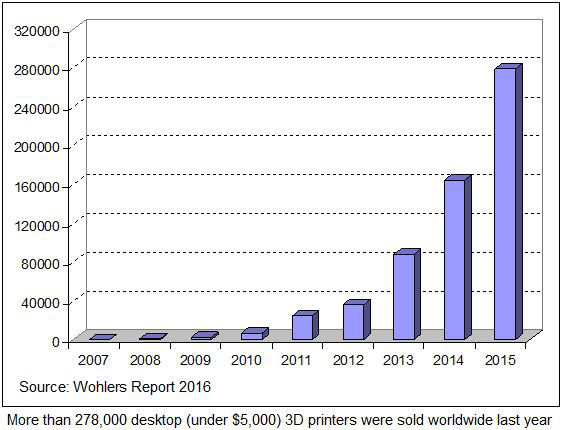
\includegraphics[width=400px]{https://raw.githubusercontent.com/fabbiocrux/Figures/main/AM/3DP-growth} 

}

\caption{Nombre de ventes de machines open-source. Source Wohlers Report 2016}\label{fig:3dp-growth}
\end{figure}

Grâce à la démocratisation de ces projets, la fabrication de produits
complexes et de grande valeur est devenue accessible à tous
(\protect\hyperlink{ref-Kostakis2013}{Kostakis and Papachristou, 2014};
\protect\hyperlink{ref-Pearce2014k}{Pearce, 2014}). Le tableau
@ref(tab:table-1) compare certaines caractéristiques de la fabrication
additive open-source et commerciale. Les principaux éléments qui
expliquent la croissance exponentiel et l'intérêt de ce types de
machines pour un grand public sont: le coût réduit par rapport aux
machines commerciales, la disponibilité de l'information technique, et
le support de tout une communauté connectée sur l'internet autour de
cette technologie. Ces éléments clés ont permis déclencher un processus
de démocratisation de cette technologie. De plus, cette technologie peut
avoir un impact positif sur les communautés comme les laboratoires
universitaires, les écoles, et ouvrir de nouvelles dimensions à
l'enseignement des sciences qui peut avoir un impact marqué dans les
pays en voie de développement (\protect\hyperlink{ref-Irwin2014}{Irwin
et al., 2014}).

\providecommand{\docline}[3]{\noalign{\global\setlength{\arrayrulewidth}{#1}}\arrayrulecolor[HTML]{#2}\cline{#3}}

\setlength{\tabcolsep}{2pt}

\renewcommand*{\arraystretch}{1.5}

\begin{longtable}[c]{|p{1.00in}|p{2.00in}|p{2.00in}}

\caption{Comparaison des machines open-source et commerciales.}\\

\hhline{~~~}

\multicolumn{1}{!{\color[HTML]{000000}\vrule width 0pt}>{\cellcolor[HTML]{CFCFCF}\raggedright}p{\dimexpr 1in+0\tabcolsep+0\arrayrulewidth}}{\fontsize{11}{11}\selectfont{\textcolor[HTML]{000000}{\textbf{ }}}} & \multicolumn{1}{!{\color[HTML]{000000}\vrule width 0pt}>{\cellcolor[HTML]{CFCFCF}\raggedright}p{\dimexpr 2in+0\tabcolsep+0\arrayrulewidth}}{\fontsize{11}{11}\selectfont{\textcolor[HTML]{000000}{\textbf{FA Open-Source}}}} & \multicolumn{1}{!{\color[HTML]{000000}\vrule width 0pt}>{\cellcolor[HTML]{CFCFCF}\raggedright}p{\dimexpr 2in+0\tabcolsep+0\arrayrulewidth}!{\color[HTML]{000000}\vrule width 0pt}}{\fontsize{11}{11}\selectfont{\textcolor[HTML]{000000}{\textbf{FA Commercial}}}} \\



\endfirsthead

\hhline{~~~}

\multicolumn{1}{!{\color[HTML]{000000}\vrule width 0pt}>{\cellcolor[HTML]{CFCFCF}\raggedright}p{\dimexpr 1in+0\tabcolsep+0\arrayrulewidth}}{\fontsize{11}{11}\selectfont{\textcolor[HTML]{000000}{\textbf{ }}}} & \multicolumn{1}{!{\color[HTML]{000000}\vrule width 0pt}>{\cellcolor[HTML]{CFCFCF}\raggedright}p{\dimexpr 2in+0\tabcolsep+0\arrayrulewidth}}{\fontsize{11}{11}\selectfont{\textcolor[HTML]{000000}{\textbf{FA Open-Source}}}} & \multicolumn{1}{!{\color[HTML]{000000}\vrule width 0pt}>{\cellcolor[HTML]{CFCFCF}\raggedright}p{\dimexpr 2in+0\tabcolsep+0\arrayrulewidth}!{\color[HTML]{000000}\vrule width 0pt}}{\fontsize{11}{11}\selectfont{\textcolor[HTML]{000000}{\textbf{FA Commercial}}}} \\

\endhead



\multicolumn{1}{!{\color[HTML]{000000}\vrule width 0pt}>{\cellcolor[HTML]{EFEFEF}\raggedright}p{\dimexpr 1in+0\tabcolsep+0\arrayrulewidth}}{\fontsize{11}{11}\selectfont{\textcolor[HTML]{000000}{Principe:}}} & \multicolumn{1}{!{\color[HTML]{000000}\vrule width 0pt}>{\cellcolor[HTML]{EFEFEF}\raggedright}p{\dimexpr 2in+0\tabcolsep+0\arrayrulewidth}}{\fontsize{11}{11}\selectfont{\textcolor[HTML]{000000}{CAD + GCode + Impression.}}} & \multicolumn{1}{!{\color[HTML]{000000}\vrule width 0pt}>{\cellcolor[HTML]{EFEFEF}\raggedright}p{\dimexpr 2in+0\tabcolsep+0\arrayrulewidth}!{\color[HTML]{000000}\vrule width 0pt}}{\fontsize{11}{11}\selectfont{\textcolor[HTML]{000000}{CAD + GCode + Impression.}}} \\





\multicolumn{1}{!{\color[HTML]{000000}\vrule width 0pt}>{\raggedright}p{\dimexpr 1in+0\tabcolsep+0\arrayrulewidth}}{\fontsize{11}{11}\selectfont{\textcolor[HTML]{000000}{Coût}}} & \multicolumn{1}{!{\color[HTML]{000000}\vrule width 0pt}>{\raggedright}p{\dimexpr 2in+0\tabcolsep+0\arrayrulewidth}}{\fontsize{11}{11}\selectfont{\textcolor[HTML]{000000}{US\$200-US\$5000}}} & \multicolumn{1}{!{\color[HTML]{000000}\vrule width 0pt}>{\raggedright}p{\dimexpr 2in+0\tabcolsep+0\arrayrulewidth}!{\color[HTML]{000000}\vrule width 0pt}}{\fontsize{11}{11}\selectfont{\textcolor[HTML]{000000}{US\$5.000 jusqu'à US\$800 K}}} \\





\multicolumn{1}{!{\color[HTML]{000000}\vrule width 0pt}>{\cellcolor[HTML]{EFEFEF}\raggedright}p{\dimexpr 1in+0\tabcolsep+0\arrayrulewidth}}{\fontsize{11}{11}\selectfont{\textcolor[HTML]{000000}{Méthodologie:}}} & \multicolumn{1}{!{\color[HTML]{000000}\vrule width 0pt}>{\cellcolor[HTML]{EFEFEF}\raggedright}p{\dimexpr 2in+0\tabcolsep+0\arrayrulewidth}}{\fontsize{11}{11}\selectfont{\textcolor[HTML]{000000}{Open design}}} & \multicolumn{1}{!{\color[HTML]{000000}\vrule width 0pt}>{\cellcolor[HTML]{EFEFEF}\raggedright}p{\dimexpr 2in+0\tabcolsep+0\arrayrulewidth}!{\color[HTML]{000000}\vrule width 0pt}}{\fontsize{11}{11}\selectfont{\textcolor[HTML]{000000}{Closed Design (Patented)}}} \\





\multicolumn{1}{!{\color[HTML]{000000}\vrule width 0pt}>{\raggedright}p{\dimexpr 1in+0\tabcolsep+0\arrayrulewidth}}{\fontsize{11}{11}\selectfont{\textcolor[HTML]{000000}{Développé par:}}} & \multicolumn{1}{!{\color[HTML]{000000}\vrule width 0pt}>{\raggedright}p{\dimexpr 2in+0\tabcolsep+0\arrayrulewidth}}{\fontsize{11}{11}\selectfont{\textcolor[HTML]{000000}{Communauté globale}}} & \multicolumn{1}{!{\color[HTML]{000000}\vrule width 0pt}>{\raggedright}p{\dimexpr 2in+0\tabcolsep+0\arrayrulewidth}!{\color[HTML]{000000}\vrule width 0pt}}{\fontsize{11}{11}\selectfont{\textcolor[HTML]{000000}{Quelques entreprises}}} \\





\multicolumn{1}{!{\color[HTML]{000000}\vrule width 0pt}>{\cellcolor[HTML]{EFEFEF}\raggedright}p{\dimexpr 1in+0\tabcolsep+0\arrayrulewidth}}{\fontsize{11}{11}\selectfont{\textcolor[HTML]{000000}{Imprimante:}}} & \multicolumn{1}{!{\color[HTML]{000000}\vrule width 0pt}>{\cellcolor[HTML]{EFEFEF}\raggedright}p{\dimexpr 2in+0\tabcolsep+0\arrayrulewidth}}{\fontsize{11}{11}\selectfont{\textcolor[HTML]{000000}{Personnalisé}}} & \multicolumn{1}{!{\color[HTML]{000000}\vrule width 0pt}>{\cellcolor[HTML]{EFEFEF}\raggedright}p{\dimexpr 2in+0\tabcolsep+0\arrayrulewidth}!{\color[HTML]{000000}\vrule width 0pt}}{\fontsize{11}{11}\selectfont{\textcolor[HTML]{000000}{Standardisé}}} \\





\multicolumn{1}{!{\color[HTML]{000000}\vrule width 0pt}>{\raggedright}p{\dimexpr 1in+0\tabcolsep+0\arrayrulewidth}}{\fontsize{11}{11}\selectfont{\textcolor[HTML]{000000}{Exemple:}}} & \multicolumn{1}{!{\color[HTML]{000000}\vrule width 0pt}>{\raggedright}p{\dimexpr 2in+0\tabcolsep+0\arrayrulewidth}}{\fontsize{11}{11}\selectfont{\textcolor[HTML]{000000}{Projet RepRap}}} & \multicolumn{1}{!{\color[HTML]{000000}\vrule width 0pt}>{\raggedright}p{\dimexpr 2in+0\tabcolsep+0\arrayrulewidth}!{\color[HTML]{000000}\vrule width 0pt}}{\fontsize{11}{11}\selectfont{\textcolor[HTML]{000000}{Stratasys}}} \\



\end{longtable}

\hypertarget{recyclage-de-polymuxe8res}{%
\subsection{Recyclage de polymères}\label{recyclage-de-polymuxe8res}}

Le développement de matériaux polymères a permis la fabrication d'une
large gamme de produits peu coûteux, de faible poids et de haute
performance et il est devenu un élément essentiel du développement
technologique et sociétal (\protect\hyperlink{ref-Andrady2009}{Andrady
and Neal, 2009}). Cependant, l'un des principaux problèmes est l'impact
environnemental des résidus de plastique en raison de leur longévité qui
peut atteindre plusieurs décennies
(\protect\hyperlink{ref-Hopewell2009}{Hopewell et al., 2009}).

Dans l'écologie industrielle des polymères, différentes stratégies ont
été étudiées pour la gestion des déchets plastiques, allant de la
réutilisation et du recyclage (Mécanique, Chimique) jusqu'à des
processus de thermolyse / récupération
(\protect\hyperlink{ref-AlSalem2009}{Al-Salem et al., 2009};
\protect\hyperlink{ref-Clift1997}{Clift, 1997};
\protect\hyperlink{ref-Hopewell2009}{Hopewell et al., 2009}).

Dans le contexte de recyclage des thermoplastiques, une des stratégies
développées pour le traitement de déchets est le recyclage mécanique. Le
recyclage mécanique est défini comme un processus qui permet de
réutiliser directement des déchets plastiques dans le procédé de
fabrication des nouveaux produits. Dans ce cas, il n'y a pas de
destruction significative de la structure chimique du polymère, tout au
plus quelques modifications de ses propriétés physiques
(\protect\hyperlink{ref-AlSalem2009}{Al-Salem et al., 2009};
\protect\hyperlink{ref-Fisher2004}{Fisher, 2004};
\protect\hyperlink{ref-Hopewell2009}{Hopewell et al., 2009};
\protect\hyperlink{ref-Perugini2005}{Perugini et al., 2005};
\protect\hyperlink{ref-Robin2012}{Robin, 2012}).

En ce sens, le couplage de tests de caractérisation avec de multiples
procédés d'extrusion ou de moulage par injection est une approche
éprouvée pour évaluer la recyclabilité de matériaux polymères afin de
simuler le cycle de vie prolongé des produits recyclés. La figure
@ref(fig:Mechanical-Recycling-Fr) présente un schéma générale de cette
approche:

\begin{figure}

{\centering 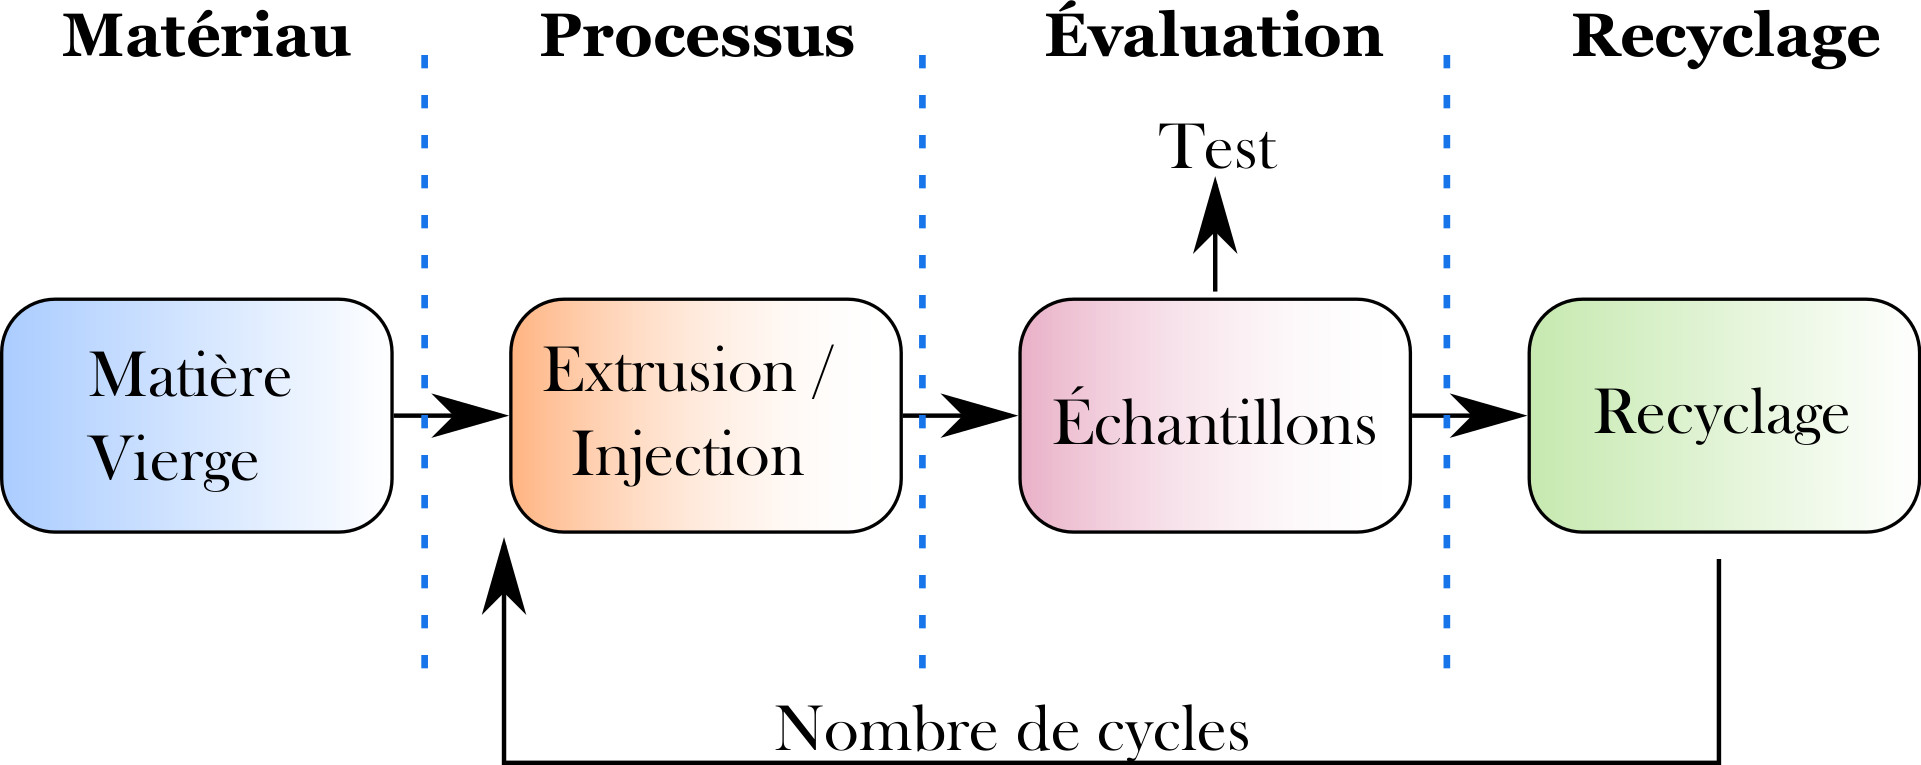
\includegraphics[width=300px]{https://raw.githubusercontent.com/fabbiocrux/Figures/main/Recycling/fr/Multiple-Processing} 

}

\caption{Mechanical recycling steps for the case of fabrication of recycled filament.}\label{fig:Mechanical-Recycling-Fr}
\end{figure}

Dans ce modèle, une phase de départ est de considérer l'étude d'une
\emph{Matière Vierge}. Une autre considération à remarquer est
l'évaluation de la matière en circuit fermé, dont il n'y a pas d'ajout
supplementaire de matière une fois le processus de recyclage commence.
La dégradation de la matière est directement liée au procédé utilisé et
a la quantité de cycles étudiés dans le recyclage. Il est nécessaire de
définir l'étape \emph{Évaluation} afin d'avoir une quantification des
propriétés du matériau recyclé. Dans le cas de matière plastique
recyclé, \protect\hyperlink{ref-Karlsson2004}{Karlsson}
(\protect\hyperlink{ref-Karlsson2004}{2004};
\protect\hyperlink{ref-Vilaplana2008}{Vilaplana and Karlsson, 2008}) ont
identifié trois axes majeurs pour l'évaluation de la qualité qui peuvent
être résumées de la manière suivante:

\begin{figure}

{\centering 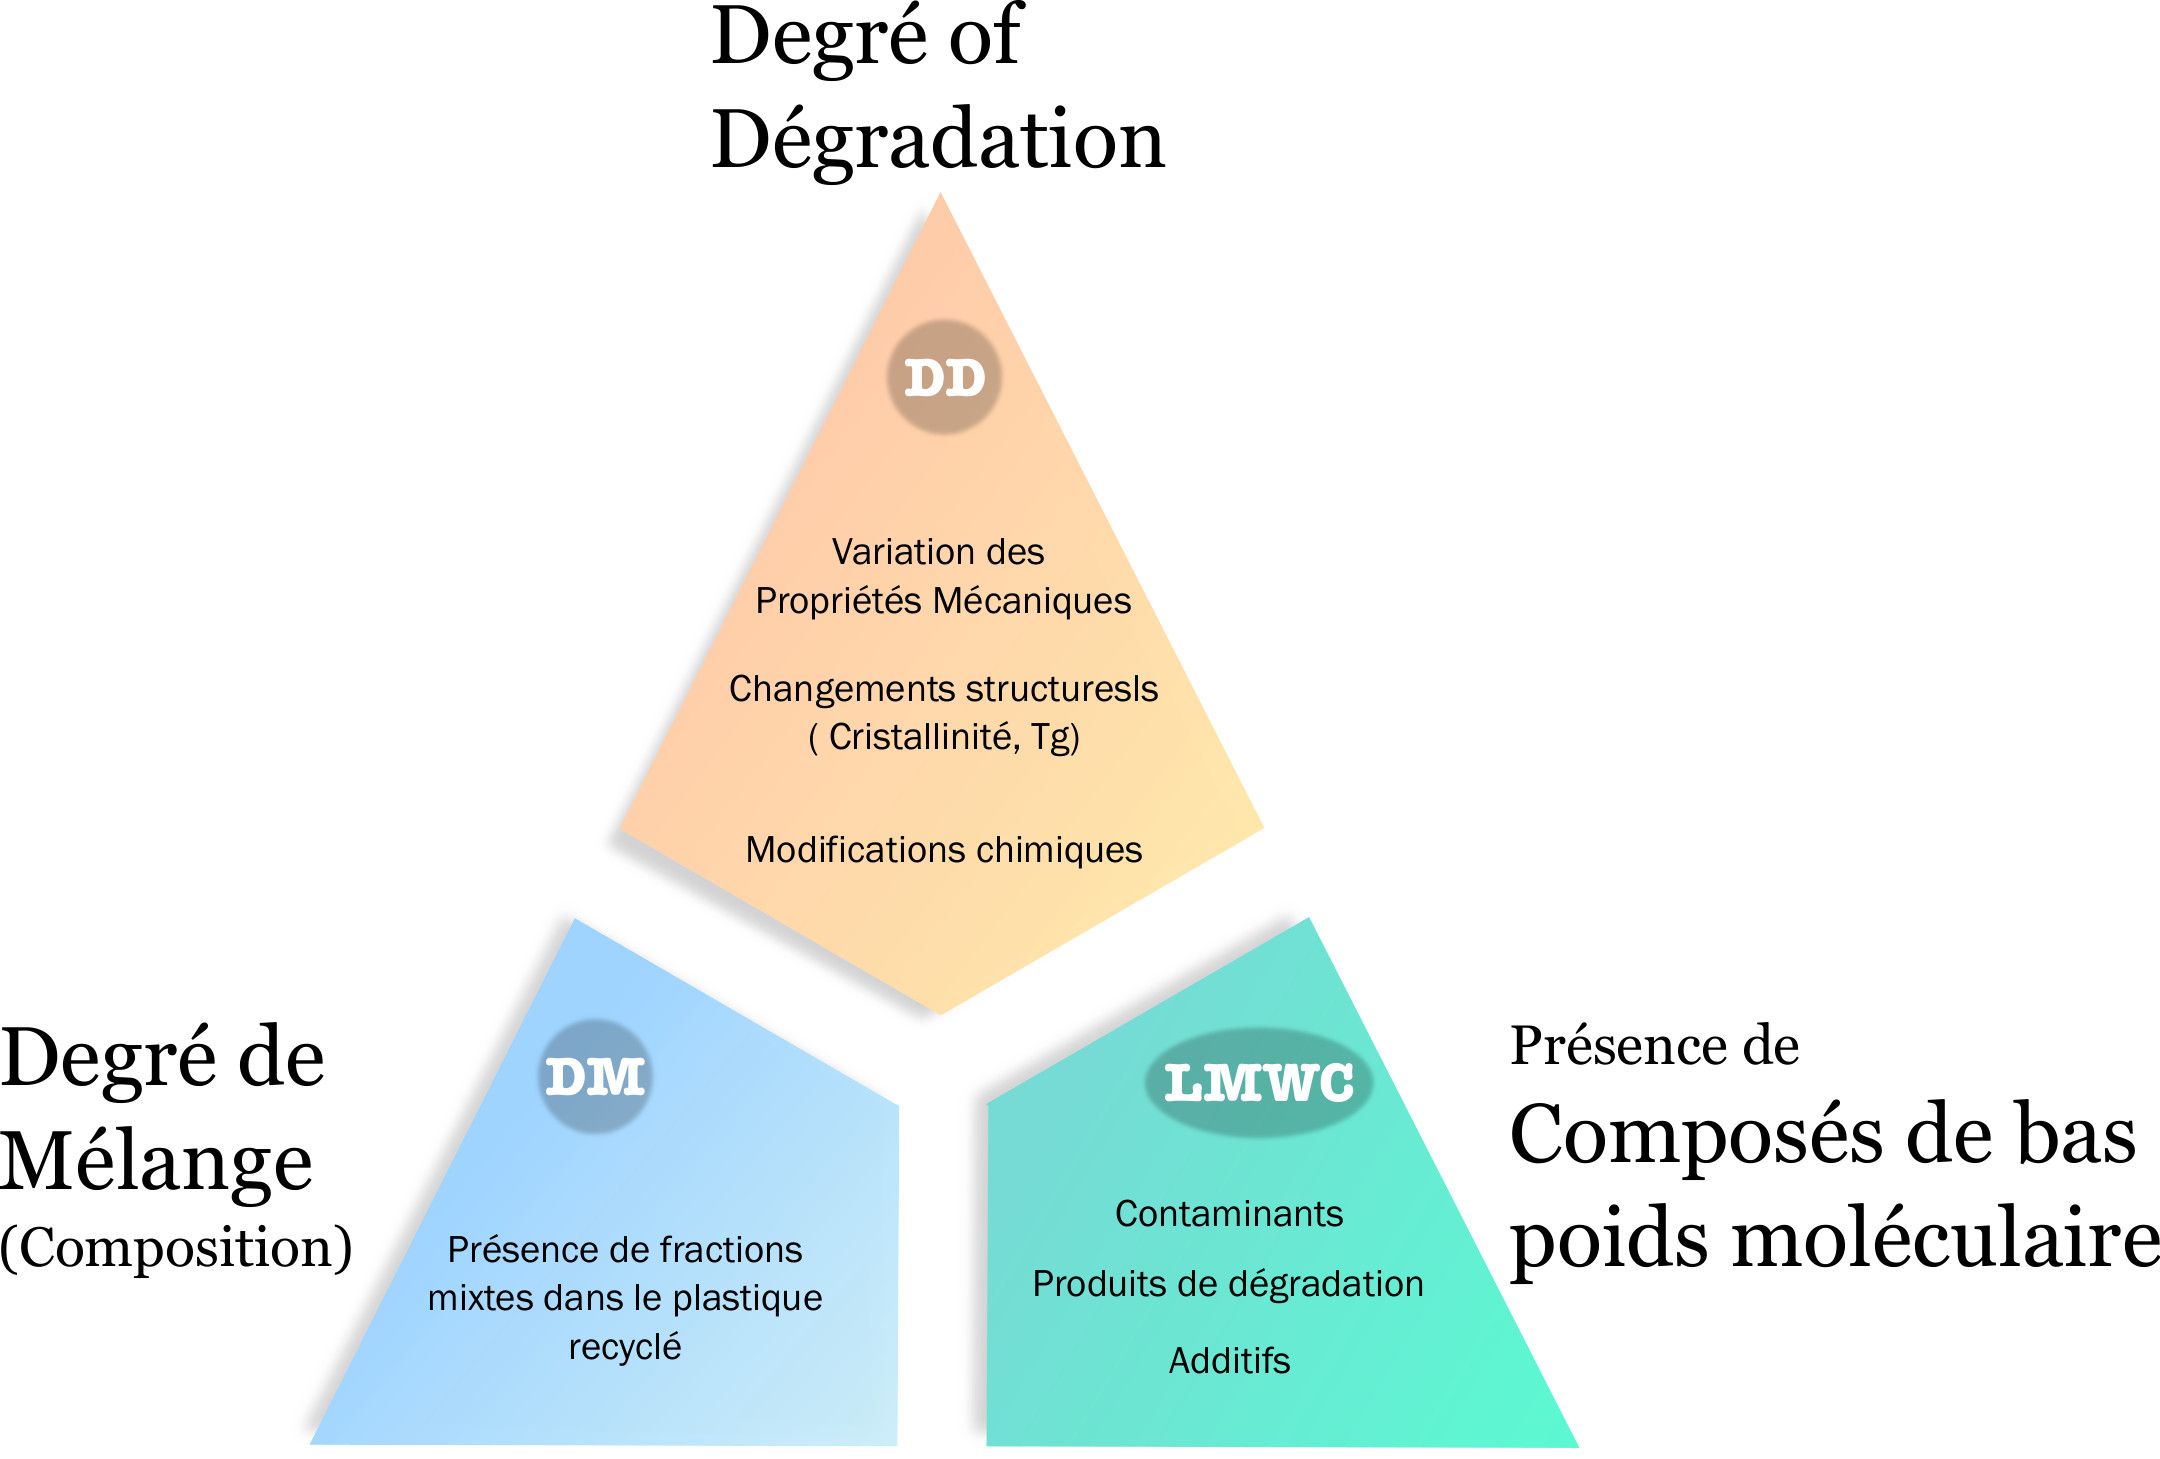
\includegraphics[width=300px]{https://raw.githubusercontent.com/fabbiocrux/Figures/main/Recycling/fr/Quality-Recycling} 

}

\caption{Cadre d'évaluation de la matière plastique recyclé.}\label{fig:Quality-Recycling-Fr}
\end{figure}

\begin{description}
\item[\emph{Degré de Mélange (DM):}]
Cet axe mesure la présence de types de polymères et d'impuretés dans le
matériau.
\item[\emph{Composés de bas poids moléculaire (LMWC):}]
Cet axe fait référence à la présence de contaminants, additifs et
d'autres éléments dans la matrice. Il est importante afin de répondre
aux exigences législatives.
\item[\emph{Degré de dégradation (DD):}]
Cet axe détermine l'évolution de la dégradation du polymère à l'échelle
macro/microscopique due au procédés de fabrication et à la durée de vie.
\end{description}

Le travaux de \protect\hyperlink{ref-Badia2016}{Badia and Ribes-Greus}
(\protect\hyperlink{ref-Badia2016}{2016}) présentent une caractérisation
multi-niveaux complète dans lequel sont représentées les différentes
axes d'analyse (\emph{DM, LMWC, DD}), ainsi que les techniques
analytiques couramment utilisées pour tester l'état de performance et /
ou de dégradation du matériau résultant. Enfin, en fonction de la (ou
les) propriété(s) qui seront analysées lors du processus de recyclage
mécanique, de protocoles expérimentaux adéquats peuvent être mis en
œuvre. Finalement, une étape de recyclage est caractérisé a fin de
pouvoir réutiliser la matière.

\hypertarget{le-recyclage-dans-la-fabrication-additive}{%
\section{Le Recyclage dans la Fabrication
Additive}\label{le-recyclage-dans-la-fabrication-additive}}

Les possibilités et les caractéristiques de la FA ont été présentées.
Nous rappelons que le but principal de cette chapitre est d'avoir une
meilleure compréhension du processus de recyclage des polymères afin
d'établir une option de gestion durable des déchets pour cette
technologie de FA open-source. Pour cela, il est essentiel de connaitre
les avances en recherche et le développement de l'utilisation de la
matière recyclé dans les technologies de la FA. Nous concentrons la
recherche sur le recyclage des polymères utilisés pour les machines
open-source. De la même façon, le but est d'identifier les
développements au niveau expérimental/machine et de recherche
méthodologique pour comprendre la faisabilité de ce processus.

En utilisant une totale de 120 articles depuis 2009 jusqu'à 2020,
\protect\hyperlink{ref-CruzSanchez2020}{Cruz Sanchez et al.}
(\protect\hyperlink{ref-CruzSanchez2020}{2020}) a fait une revue
systématique de la littérature en identifiant des élements clés sur le
recyclage (type de matière, protocole d'évaluation de la qualité,
propriétés dans l'impression) des études pour les différent technologies
de la FA qui utilisent des matière thermoplastiques. Ces éléments
permettent de comprendre la viabilité de l'utilisation de matériaux
recyclés.

Un première résultat de la revue est la mise en évidence que les études
de recyclabilité dans le contexte des procédés de FA comme SLA restent
encore une champ de recherche à explorer. Par contre, plusieurs
propositions ont été identifiés dans les procédés Selective Laser
Sintering (SLS) et FFF.

Dans le cadres des technologies FA commercial, des méthodologies de
recyclage ont été identifiés afin d'évaluer l'évolution de la matière
première que n'a pas été sintérise lors du processus d'impression SLS.
\protect\hyperlink{ref-Raugel2015}{Nandwana et al.}
(\protect\hyperlink{ref-Raugel2015}{2016}) explicitent formellement une
méthodologie utilisée pour évaluer le recyclage des poudres métalliques
dans le procédé EBM. Dans le cas de polymère,
\protect\hyperlink{ref-Dotchev2009}{Dotchev and Yusoff}
(\protect\hyperlink{ref-Dotchev2009}{2009}) ont présenté une approche
méthodologique pour évaluer les bonnes pratiques établies pour le
recyclage des poudres dans le frittage de poudre (SLS), en utilisant du
polyamide (nylon).

Dans le cadre de la FA open-source, un des concept importants à
souligner est celui du \textbf{recyclage distribué}. Ce concept consiste
en l'utilisation de déchet plastique pour les transformer en matière
première pour l'imprimante 3D grâce au développement des extrudeuses
issues aussi de l'open-source. Ce couplage des imprimantes 3D avec le
dévelopment des extrudeuses a été exploré comme une nouvelle approche
prospective afin d'optimiser la matière première pour ces machines.
Certains projets tels que Precious plastic\footnote{\protect\hyperlink{http:ux2fux2fpreciousplastic.comux2f}{http://preciousplastic.com/}}
(\protect\hyperlink{ref-Hakkens2016}{Hakkens, 2016}), Plastic
Bank\footnote{\protect\hyperlink{http:ux2fux2fplasticbank.orgux2f}{http://plasticbank.org/}}
sont basés sur ce concept. La figure @ref(fig:slr-methodology) presente
le système technique qui doit être viabilisé pour le dévelopement d'un
circuit court afin d'utiliser la technologie d'impression 3D comme un
vecture de valorisation des déchets à petit échelle.

\begin{figure}

{\centering 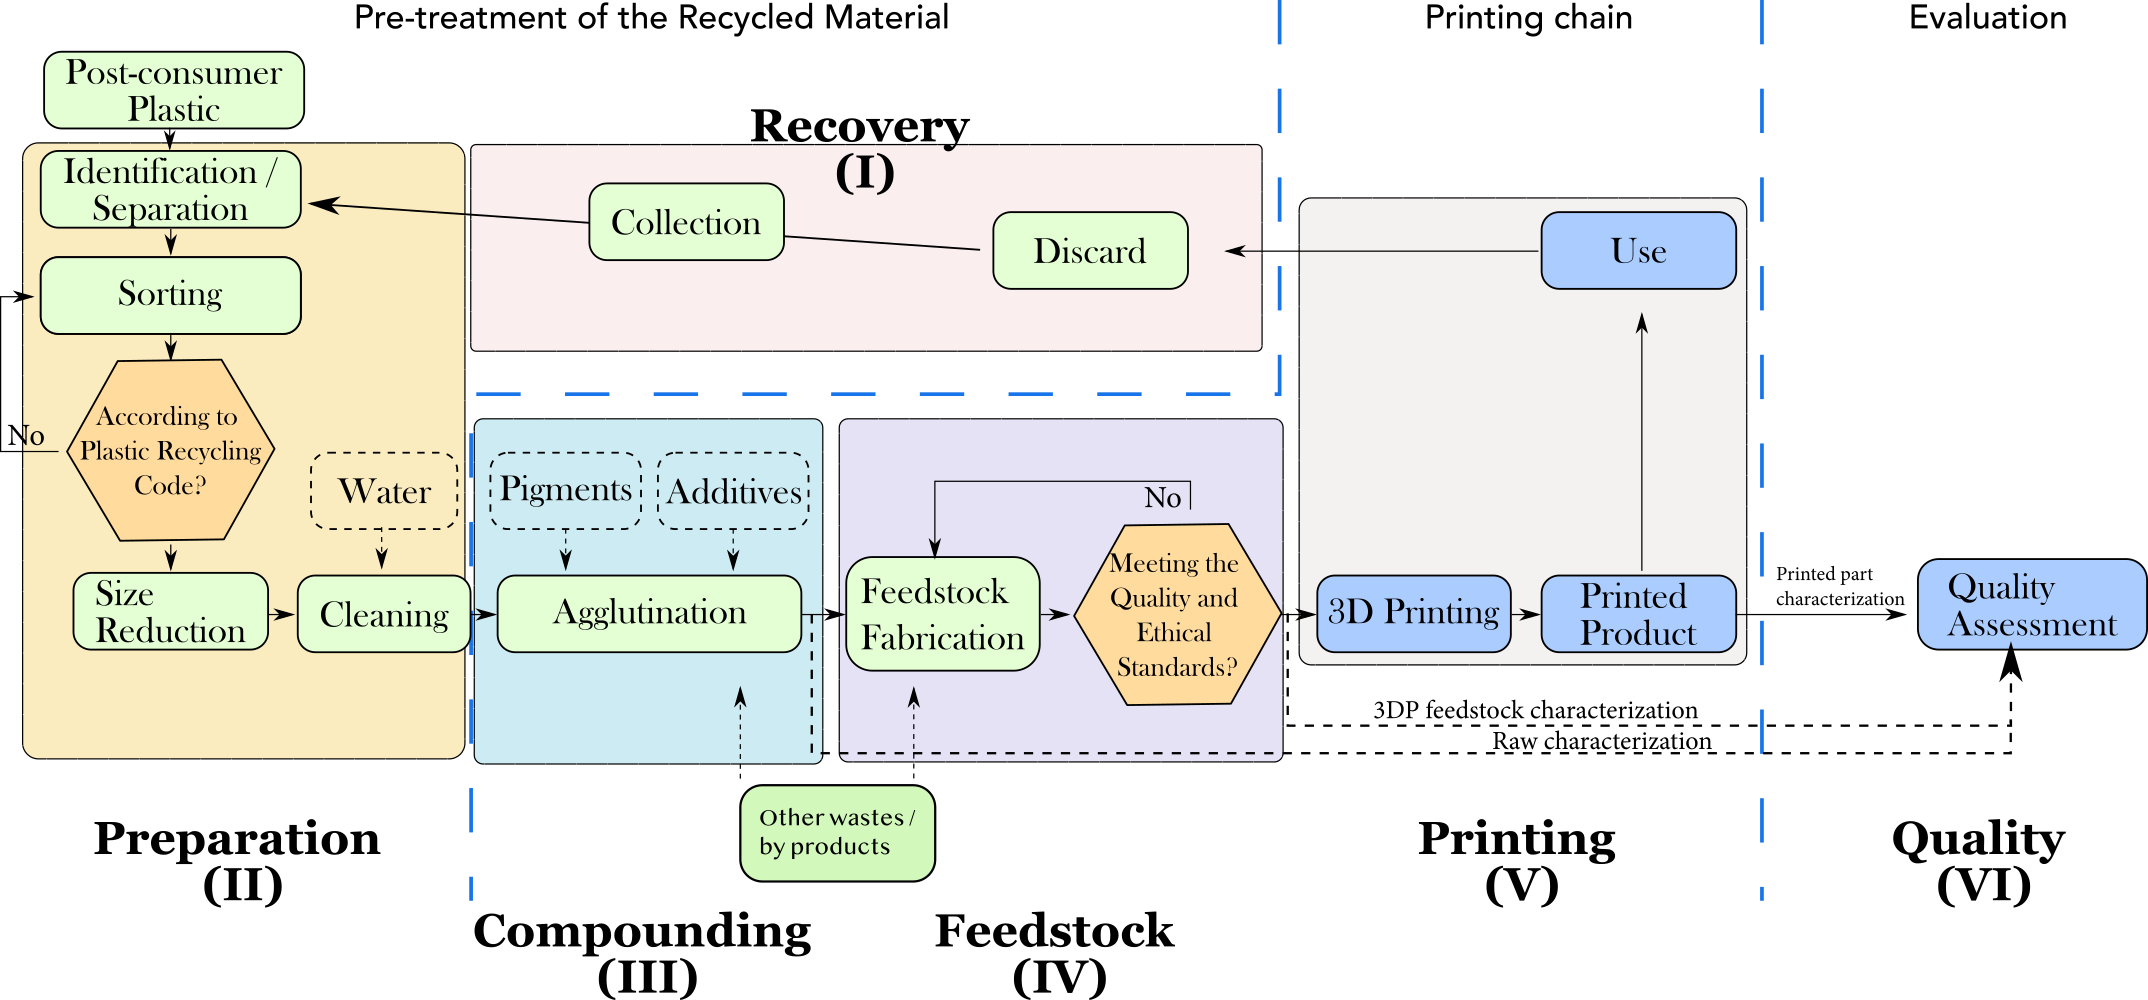
\includegraphics[width=1\linewidth]{https://raw.githubusercontent.com/fabbiocrux/Figures/main/DRAM/DRAM-10} 

}

\caption{Méthodologie de revue systématique de la littérature. Adaptée de @Kitchenham2007.}\label{fig:slr-methodology}
\end{figure}

L'intérêt principal de cette approche est la réduction des coûts et des
émissions de gaz à effet de serre liés à la collecte et au transport des
déchets ainsi qu'à l'impact environnemental de la fabrication de pièces
en plastique sur mesure. Cette approche de \textbf{recyclage des
polymères distribués} pourrait être une alternative supplémentaire au
\textbf{recyclage centralisé classique} des polymères
(\protect\hyperlink{ref-Baechler2013}{Baechler et al., 2013};
\protect\hyperlink{ref-Feeley2014}{Feeley et al., 2014};
\protect\hyperlink{ref-Anzalone2013}{Kreiger et al., 2013};
\protect\hyperlink{ref-Kreiger2014}{Kreiger et al., 2014};
\protect\hyperlink{ref-Kreiger2013}{Kreiger and Pearce, 2013}). Compte
tenu de l'adoption croissante significative de la FA open-source,
l'approche du recyclage distribué des polymères pourrait être très
pertinente car les taux actuels de recyclage sont particulièrement
faibles.

D'un point de vue économique, les coûts de filaments commerciaux se
situent entre \(\$18.86\) et \(\$175.20\) par kg, qui est de 20 à 200
fois supérieur au coût du plastique brut.
\protect\hyperlink{ref-Wittbrodt2013}{Wittbrodt et al.}
(\protect\hyperlink{ref-Wittbrodt2013}{2013}) et
\protect\hyperlink{ref-Kreiger2014}{Kreiger et al.}
(\protect\hyperlink{ref-Kreiger2014}{2014}) ont prouvé la faisabilité
économique d'un modèle distribué avec le recyclage local des matières
plastiques (filament recyclé) pour les imprimantes OS 3D dans lequel
\(1 kg\) de filament recyclé a été fabriqué à partir d'environ 20
bouteilles de lait pour moins de 10 cents US en utilisant le prototype
d'extrudeuse open-source appelée «Recyclebot». Concernant l'aspect
énergétique, \protect\hyperlink{ref-Kreiger2013}{Kreiger and Pearce}
(\protect\hyperlink{ref-Kreiger2013}{2013}) et
\protect\hyperlink{ref-Baechler2013}{Baechler et al.}
(\protect\hyperlink{ref-Baechler2013}{2013}) ont travaillé sur le
concept pour le recyclage des déchets de polymères de grande valeur, où
les économies se situaient entre 69 \% et 82 \% d'énergie intrinsèque
pour le recyclage distribué par rapport à l'approche centralisée de
recyclage traditionnel. Par conséquent, il existe un intérêt dans le
recyclage de matériaux polymères pour un contexte d'impression 3D en
open source.

Cependant, afin de comprendre le processus de recyclage des polymères
pour établir une option de gestion durable des déchets pour cette
technologie de FA open-source, il faut prendre en compte deux éléments
fondamentaux: 1) Vu la nature open-source des machines, il est
nécessaire établir une caractérisation afin de comprendre la performance
de ces machines par rapport à l'ensemble de procédés de fabrication. En
outre, la relation entre les paramètres de fabrication / procédé /
propriétés obtenus doit être clarifié.

\begin{enumerate}
\def\labelenumi{\arabic{enumi})}
\setcounter{enumi}{1}
\tightlist
\item
  Une fois la performance des machines OS est caractérisé, nous nous
  intéressons pour le processus de dégradation des propriétés
  physico-chimiques du polymère à chaque cycle de recyclage, à la
  manière de traiter et de valider la pertinence et le nombre de fois
  qu'un matériau peut être recycle
\end{enumerate}

\hypertarget{muxe9thodologie-pour-recycler-des-polymuxe8res-pour-la-fabrication-additive}{%
\section{Méthodologie pour évaluet le potentiel de récyclabilité des
polymères pour la fabrication
additive}\label{muxe9thodologie-pour-recycler-des-polymuxe8res-pour-la-fabrication-additive}}

Basée sur les caractéristiques du processus de recyclage mécanique, nous
proposons d'adapter un méthodologie systématique pour évaluer la
dégradation des polymères thermoplastiques dans la chaîne des procédés
de l'impression 3D. Cette méthodologie permet de comparer la dégradation
de la matière en utilisant un procédé \emph{standard} de fabrication
(e.g.~injection) par rapport à l'impression. En plus, un deuxième but
est de quantifier l'impact du procédé d'impression lui-même sur la
dégradation de la matière. La figure @ref(fig:Recycling-Methodology-Fr)
montre la méthodologie proposée.

\begin{figure}

{\centering \includegraphics[width=1\linewidth]{https://raw.githubusercontent.com/fabbiocrux/Figures/main/Recycling/fr/Recycling-Methodology} 

}

\caption{Méthodologie pour évaluer la faisabilité de recyclage dans la FA open-source.}\label{fig:Recycling-Methodology-Fr}
\end{figure}

CHaque étape sera explicité dans les sous-section suivantes

\hypertarget{etape-1-duxe9finition-du-matuxe9riau}{%
\subsection{Etape 1: ``Définition du
matériau''}\label{etape-1-duxe9finition-du-matuxe9riau}}

Le but principale de cette étape, appelé \textbf{\emph{``Définition du
matériau''}} (figure @ref(fig:Recycling-Methodology-Fr) est la
caractérisation du la matière première à étudier. Les caractéristiques
donnés par le fournisseur du polymère doivent être prises en compte pour
l'établissement initial des conditions opératoires.

De même, la quantité de matière nécessaire total pour l'étude globale
doit être estimée. Cependant, dans le but d'avoir uneestimation réelle
de la quantité de matière, il est nécessaire de prendre en compte des
éléments qui seront définis dans les étapes subséquentes. Ces éléments
sont:

\begin{itemize}
\tightlist
\item
  Idéntification des propriétés du matériau à étudier lors du processus
  de recyclage (étape détaillée dans le
  \protect\hyperlink{Step2}{step2})
\item
  Définition des chaînes de processus de recyclage nécessaires pour la
  caractérisation de la matière dégradé (étape détaillée dans le
  \protect\hyperlink{Step3}{step 3})
\item
  Définition du nombre de cycles à tester.
\item
  Estimation de la perte de matière éventuelle pendant les cycles de
  recyclage, afin de prévoir dès le début de l'expérimentation les
  quantités adéquates de matière.
\end{itemize}

\hypertarget{Step2}{%
\subsection{Etape 2: ``Procédés de fabrication''}\label{Step2}}

Cette étape est divisée en deux parties:

\begin{enumerate}
\def\labelenumi{\arabic{enumi}.}
\tightlist
\item
  \textbf{\emph{"Chaînes de processus de recyclage'}}: Il s'agit de
  l'identification des chaînes de processus de recyclage qui seront
  utilisées pour la caractérisation des propriétés du polymère recyclé.
  Afin de mettre en évidence les effets des différents procédés sur le
  matériau, au moins quatre chaînes de recyclage sont nécessaires pour
  comparer la dégradation du matériau:
\end{enumerate}

\begin{itemize}
\item
  \emph{Référence:} Il est utilisé comme une référence de la dégradation
  pour le matériau recyclé.
\item
  \emph{3D Printing:} Il est utilisé pour évaluer la dégradation du
  matériau à la suite du processus d'impression 3D avec des échantillons
  réalisés à l'aide d'une imprimante 3D avec des paramètres établis.
\item
  \emph{Feedstock:} Il est utilisé pour évaluer l'impact de la
  dégradation dû à la fabrication de la matière première pour les
  machines d'impression 3D considérées (c'est-à-dire les filament, les
  granules, la poudre, etc ...).
\item
  \emph{3DP (Référence):} Il est utilisé pour évaluer la dégradation du
  matériau dû au processus d'impression 3D en utilisant l'équipement
  standard.
\end{itemize}

En outre, plusieurs éléments caractéristiques mécaniques, thermiques,
rheologiques et morphologiques peuvent illustrer la dégradation du
polymère (\protect\hyperlink{ref-Vilaplana2007}{Vilaplana et al., 2007};
\protect\hyperlink{ref-Vilaplana2008}{Vilaplana and Karlsson, 2008}).
Pendant cette étape, l'expérimentateur doit déterminer son choix, en
sélectionnant les propriétés qui seront étudiées par le processus de
recyclage.

\begin{enumerate}
\def\labelenumi{\arabic{enumi}.}
\setcounter{enumi}{1}
\tightlist
\item
  \textbf{\emph{``Préparation de la matière première pour l'impression
  3D''}}: Le but de cette étape est d'identifier le(s) procédé(s) requis
  pour la fabrication de la matière première pour l'imprimante. Donc, la
  caractérisation de ces procédés et l'établissement des conditions
  opératoires est indispensable afin de définir les différent
  propriétés. En plus, une définition de la qualité de la matière
  obtenue est essentiel afin de garantir la qualité pendant le processus
  d'impression.
\end{enumerate}

\hypertarget{Step3}{%
\subsection{Etape 3: ``Fabrication des échantillons''}\label{Step3}}

Il y a deux buts principaux dans cette étape:

\begin{enumerate}
\def\labelenumi{\arabic{enumi}.}
\tightlist
\item
  D'abord, deux types de procédés sont proposés afin de comparer la
  dégradation de la matière: les procédés \emph{Standard} et
  \emph{l'Impression 3D}:
\end{enumerate}

\begin{itemize}
\item
  \emph{``Standard''}: Ce procédé servira de référence pour comparer les
  résultats obtenus de dégradation avec le procédé d'impression 3D. Il
  est nécessaire de caractériser l'équipement et définir les conditions
  opératoires à utiliser pour la fabrication des échantillons qui seront
  le référence de dégradation. C'est la raison pour laquelle, il est
  impératif d'identifier les normes internationales par rapport aux
  propriétés choisies dans le étape précédente
  (\protect\hyperlink{Step2}{Step 2- Processus de référence}).
\item
  \emph{``Impression 3D''}: Dans un premier moment, le but est de
  caractériser l'imprimante open-source utilisé dans l'expérimentation.
  Dans un deuxième moment, la définition des paramètres de fabrication
  pour les échantillons. Une revue de la littérature sur la propriété
  sélectionnée dans le contexte de fabrication additive commerciale peut
  donner un aperçu initial des paramètres importants à considérer.
\end{itemize}

\hypertarget{Step4}{%
\subsection{Etape 4: ``Évaluation''}\label{Step4}}

Le principaux objectifs de cette étape sont la définition des paramètres
qui décrivent les propriétés ciblées et la définition de l'équipement
sélectionné pour l'évaluation. Les tests sont effectués afin de
recueillir les données selon les procédures internationales, et en
considérant également l'ensemble des échantillons selon les chaînes de
recyclage proposés.

\hypertarget{Step5}{%
\subsection{Etape 5: ``Recyclage''}\label{Step5}}

Finalement, le but de cette étape est d'acconditionner la matière
récyclée pour le retraitement. Le processus de recyclage est réalisé
individuellement pour chaque chaîne de recyclage. Une caractérisation de
l'équipement de recyclage utilisé et une description des
caractéristiques du matériau recyclé obtenu sont réalisées.

\hypertarget{recyclage-de-lacide-polylactique-pla-pour-limpression-3d}{%
\section{Recyclage de l'Acide Polylactique (PLA) pour l'Impression
3D}\label{recyclage-de-lacide-polylactique-pla-pour-limpression-3d}}

\hypertarget{etape-1---duxe9finition-du-matuxe9riau-lacide-polylactique-pla}{%
\subsection{Etape 1 - Définition du Matériau: L'acide Polylactique
(PLA)}\label{etape-1---duxe9finition-du-matuxe9riau-lacide-polylactique-pla}}

Nous applicons la méthodologie présenté dans la figure
@ref(fig:Recycling-Methodology-Fr) à un cas particulier. Le matériau
sélectionné est l'acide polylactique (PLA) type 4043D (NatureWorks). Ce
matériau est destiné à la fabrication de matière première pour les
imprimantes 3D selon les spécifications du fabricant.

L'acide polylactique (PLA) est l'un des plus importants polymères
bio-sourcés, biodégradables et biocompatibles
(\protect\hyperlink{ref-Drumright2000}{Drumright et al., 2000};
\protect\hyperlink{ref-Henton2005}{Henton et al., 2005};
\protect\hyperlink{ref-Luckachan2011}{Luckachan and Pillai, 2011};
\protect\hyperlink{ref-Mohanty2000}{Mohanty et al., 2000};
\protect\hyperlink{ref-Soroudi2013}{Soroudi and Jakubowicz, 2013}). Le
PLA est un polyester aliphatique thermoplastique obtenue à partir des
ressources renouvelables (e.g.~pomme de terre, l'amidon du maïs, la
canne à sucre et le sucre de maïs) en usant un procédé de polymérisation
par ouverture de cycle du lactide
(\protect\hyperlink{ref-Agrawal2003}{Agrawal and Bhalla, 2003};
\protect\hyperlink{ref-Castro-Aguirre2016}{Castro-Aguirre et al., 2016};
\protect\hyperlink{ref-Hamad2013}{Hamad et al., 2013}). Le PLA offre des
potentiels avantages nombreuses pour une large gamme d'applications de
produits tels que des bouteilles, des plateaux, des conteneurs, entre
autres.

\hypertarget{etape-2---assignation-des-processus}{%
\subsection{Etape 2 - Assignation des
processus}\label{etape-2---assignation-des-processus}}

\hypertarget{processus-de-ruxe9ference}{%
\subsubsection{Processus de Réference}\label{processus-de-ruxe9ference}}

Une adaptation du processus de recyclage mécanique a été fait afin de
définir les chaînes de recyclages. La figure
@ref(fig:Recycling-Process-Chains-Fr) présente les quatre chaînes de
recyclage qui ont pour but final de qualifier la dégradation des
propriétés mécaniques dû au effet des divers procédés.

\begin{figure}

{\centering 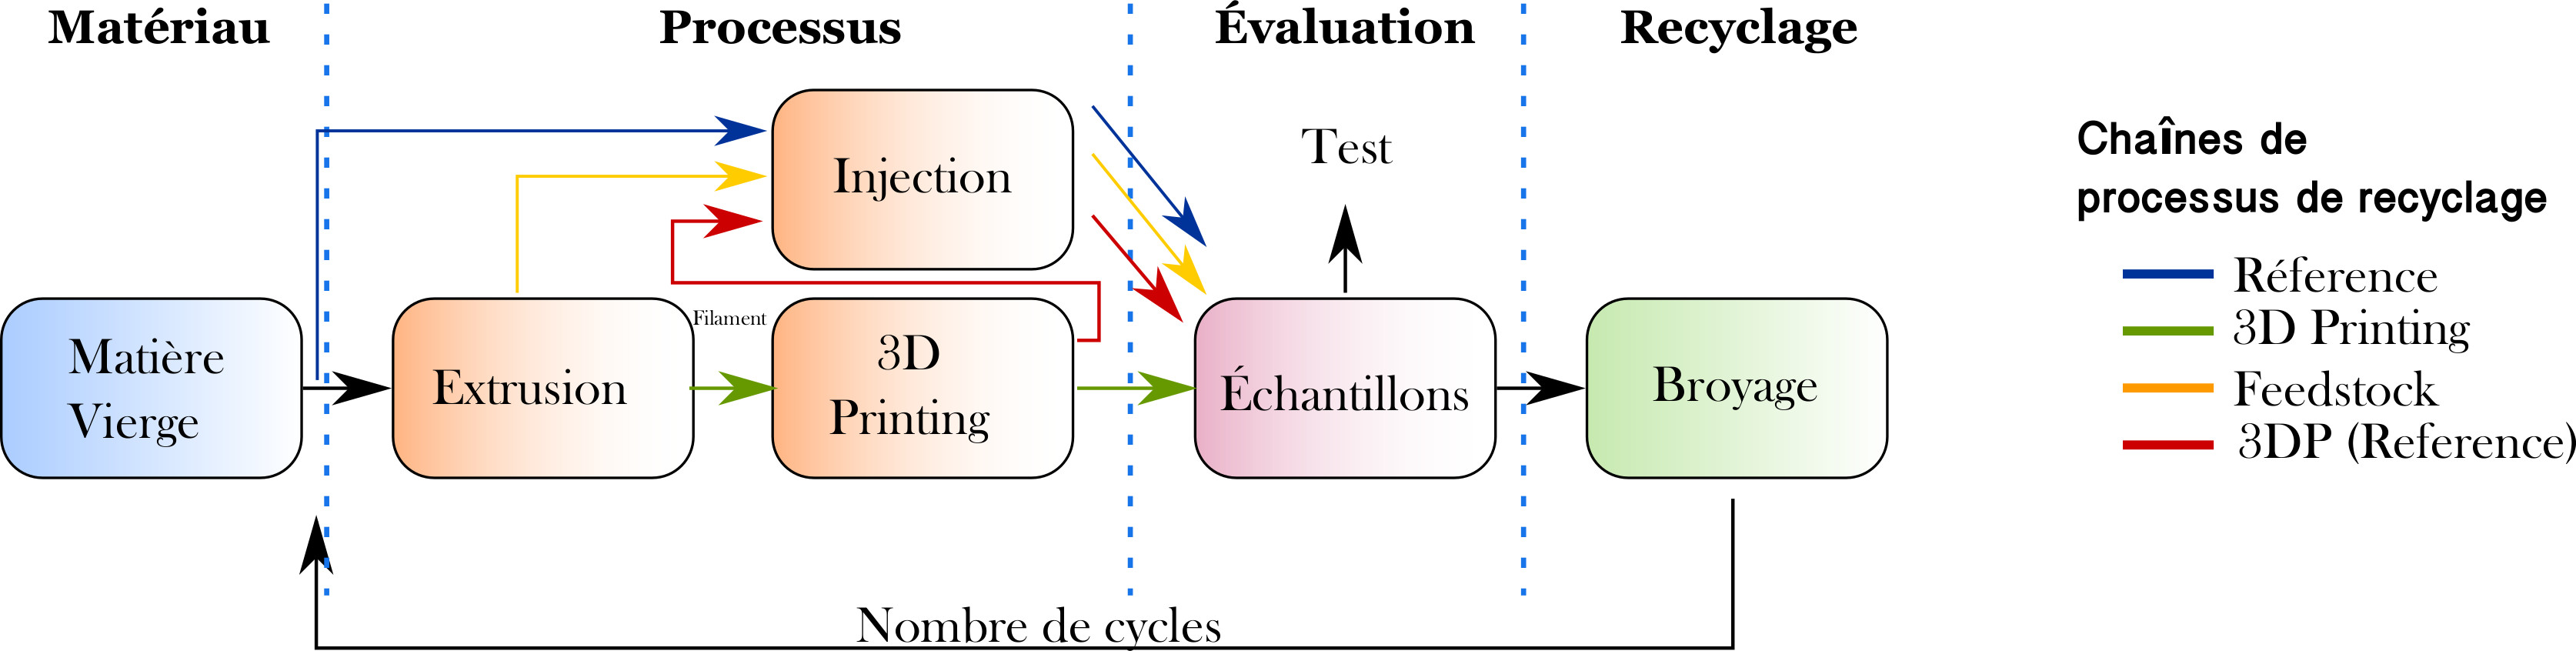
\includegraphics[width=1\linewidth]{https://raw.githubusercontent.com/fabbiocrux/Figures/main/Recycling/fr/Recycling-Process-Chains} 

}

\caption{Chaînes de recyclage pour évaluer la dégradation du matériau.}\label{fig:Recycling-Process-Chains-Fr}
\end{figure}

Nous avons défini l'étape \emph{Matériau} dans la section précédente, en
supposant que nous partons de matériaux vierges pour effectuer le
processus de recyclage. En ce qui concerne l'étape \emph{Processus},
nous supposons que le matériau sera dégradé par ces trois processus
(Injection, Extrusion et Impression 3D). Les quatre chaînes de recyclage
nous permettront de comprendre et de comparer l'impact de chaque
processus sur la dégradation du matériau.

\hypertarget{pruxe9paration-de-la-matiuxe8re-premiuxe8re-pour-limpression-3d}{%
\subsubsection{Préparation de la matière première pour l'impression
3D}\label{pruxe9paration-de-la-matiuxe8re-premiuxe8re-pour-limpression-3d}}

A cet égard, l'extrusion du polymère en monofilament peut être réalisée
par filage à chaud, qui est l'une des techniques les plus importantes
pour le traitement en continu du PLA
(\protect\hyperlink{ref-Gupta2007}{Gupta et al., 2007};
\protect\hyperlink{ref-Lim2008}{Lim et al., 2008}). Il y a certains
éléments à prendre en compte concernant les exigences relatives au
matériau de base pour les imprimantes 3D. Du point de vue des propriétés
mécaniques, il est nécessaire de s'assurer que le filament présente
certaines caractéristiques telles que:

\begin{itemize}
\tightlist
\item
  Module de flexion et résistance élevés pour permettre des opérations
  de bobinage et de débobinage en continu,
\item
  une résistance élevée à la compression pour ne pas se casser après
  être passé par les rouleaux de l'imprimante 3D, et
\item
  un module d'élasticité, des propriétés géométriques et rhéologiques
  élevés afin d'être extrudé sans effet de plissement conduisant à un
  mode de défaillance du filament.
\end{itemize}

Le paramètre sélectionné pour établir la qualité de la matière première
était la régularité du diamètre (\(\phi\)). Cette valeur est une donnée
d'entrée pour notre processus d'impression.

Pour les besoins de cette expérience, nous considérerons ce processus
comme une somme de trois systèmes, à savoir (I) le système
d'alimentation, (II) le processus d'extrusion et (III) le système de
convoyage, comme le montre la figure @ref(fig:extrusion).

\begin{figure}

{\centering 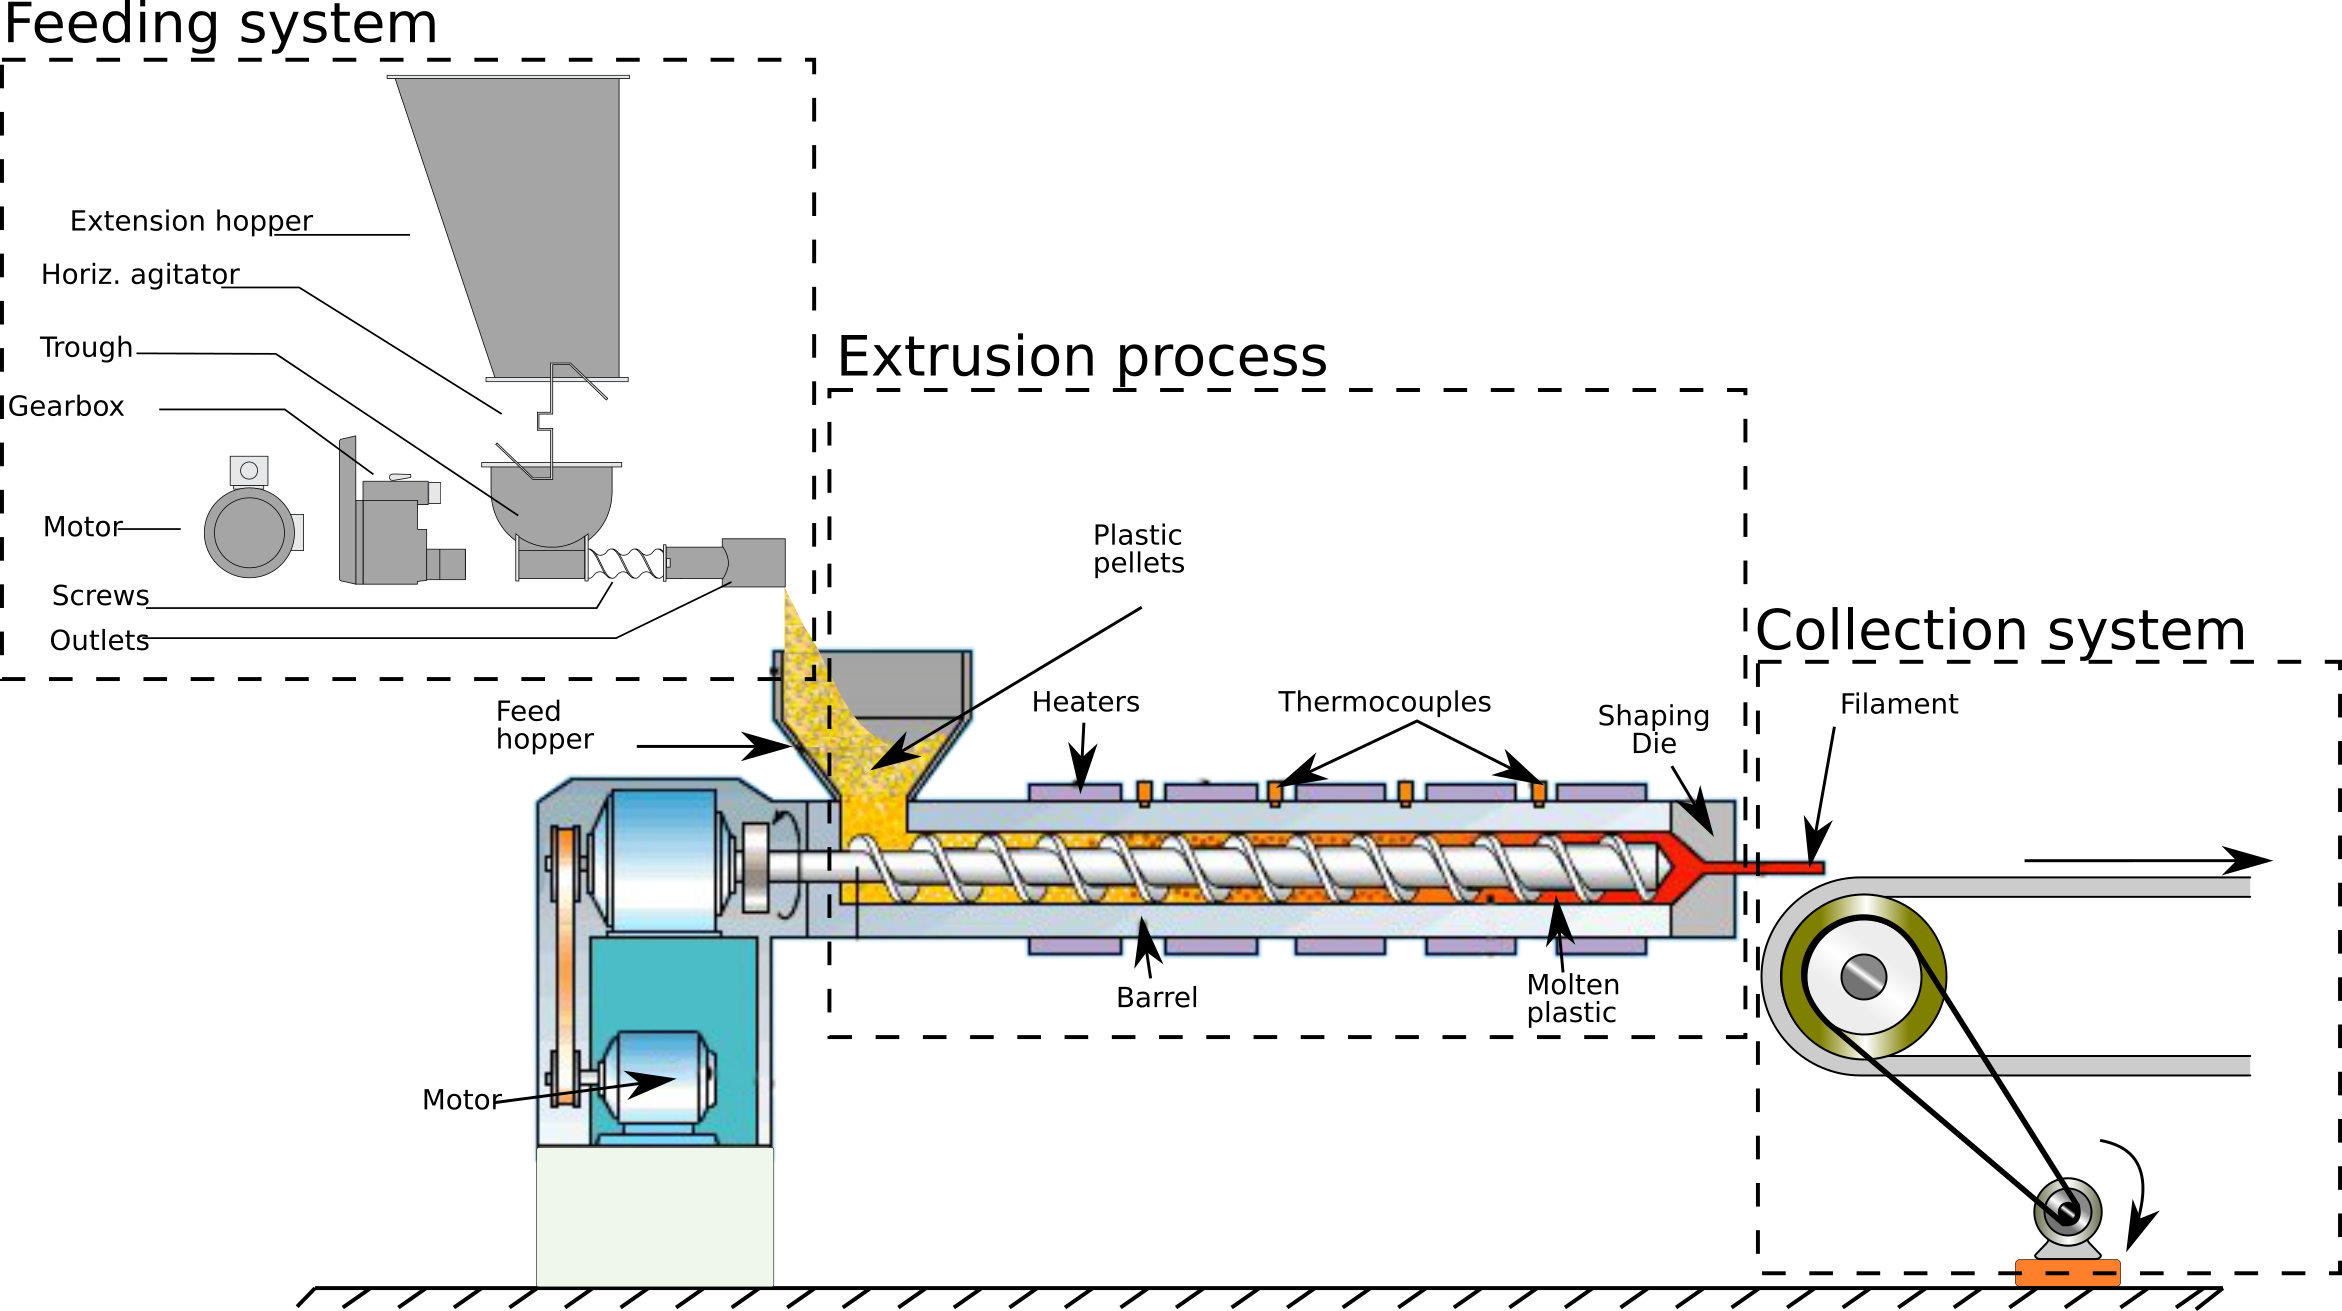
\includegraphics[width=1\linewidth]{https://raw.githubusercontent.com/fabbiocrux/Figures/main/Extrusion-process/Extrusion-process-00} 

}

\caption{Chaînes de recyclage pour évaluer la dégradation du matériau.}\label{fig:extrusion}
\end{figure}

Le système d'alimentation est réalisé à l'aide d'un alimentateur
volumétrique à double vis K-TRON (K-MV-KT20). Le débit d'alimentation
est contrôlé par la vitesse du moteur et le réducteur de l'engrenage et
un agitateur horizontal déplace doucement le matériau en vrac vers la
grande gorge, puis dans les vis. Les conditions des paramètres du
système d'alimentation sont de 100 RPM pour le moteur en utilisant une
granulométrie des granulés. La vitesse d'alimentation utilisée a été
établie à 0,53 ± 0,04 Kg/hr.

Le processus d'extrusion est réalisé afin de fabriquer le filament
utilisé dans le processus d'impression 3D. Il a été réalisé à l'aide
d'une extrudeuse à double vis conique contrarotative HAAKETM Rheomex CTW
100 OS à l'échelle du laboratoire. La plage de vitesse de fonctionnement
de cette machine est comprise entre 0 et 250 tr/min. La vitesse de la
vis a été réglée à 60 tr/min. Le profil de température sélectionné était
de 160, 170 et 180°C.

Enfin, un système de convoyeur a été adapté afin de contrôler
correctement la vitesse de reprise du filament après le processus
d'extrusion. Un système de convoyeur à bande est utilisé pour refroidir
(par convection naturelle) et collecter le filament extrudé.

\hypertarget{etape-3---fabrication-des-echantillons}{%
\subsection{Etape 3 - Fabrication des
Echantillons}\label{etape-3---fabrication-des-echantillons}}

\hypertarget{standard-micro-compounding-extrusion-et-injection}{%
\subsubsection{Standard: Micro-compounding extrusion et
injection}\label{standard-micro-compounding-extrusion-et-injection}}

Le procédé de micro-compoundage a été sélectionné comme notre procédé de
fabrication standard. Il fournit une base de comparaison entre les
différents matériaux recyclés. Les microcompounders permettent de
travailler avec une petite quantité de matériau (de 3 à 15 g) avec un
historique de traitement similaire à celui des extrudeuses à double vis
classiques.

Le matériau polymère a été traité à l'aide d'un micro-compacteur
discontinu à double vis co-rotatives à engrènement DSM Xplore d'une
capacité de 5 cm3. Le diamètre de la vis de ce dispositif va en
diminuant de 1 cm à 0,43 cm sur une longueur de 10,75 cm.

Les paramètres adoptés sont une température constante de 180°C entre la
gorge d'alimentation et la filière et une vitesse de vis de 100 tr/min
en mode contre-rotatif. Le matériau extrudé a été prélevé après un temps
de mélange de 3 minutes. Les températures de la matière fondue et du
moule étaient respectivement de 190°C et 45°C. La matière fondue a été
directement injectée à l'aide du cylindre de transfert de la machine de
moulage par injection DSM Xplore 10 ml afin d'obtenir des échantillons
mécaniques. Les pressions d'injection et de maintien ont été réglées à 9
bars pendant 30s. Les spécimens ont été soigneusement retirés du moule
après 5 min de refroidissement.

\hypertarget{impression-3d-fused-filament-fabrication-fff}{%
\subsubsection{Impression 3D: Fused Filament Fabrication
(FFF)}\label{impression-3d-fused-filament-fabrication-fff}}

L'une des principales caractéristiques de l'impression 3D à code source
ouvert est qu'elle a été un objet d'expérimentation sociale, où de
nombreux passionnés et communautés ont développé un nombre important
d'architectures de machines d'impression 3D
(\protect\hyperlink{ref-Kostakis2013}{Kostakis and Papachristou, 2014}).
Par conséquent, en raison de la nature hautement personnalisée, il
existe différentes configurations de l'architecture de la machine, ce
qui entraîne une variabilité inhérente entre les différentes imprimantes
3D. Il est nécessaire de caractériser l'imprimante 3D open source afin
d'assurer la reproductibilité des pièces imprimées
(\protect\hyperlink{ref-CruzSanchez2014}{Cruz Sanchez et al., 2014}).

La figure 1 présente les deux types d'imprimantes 3D sélectionnés pour
la fabrication des échantillons dans cette étude.

\begin{figure}

{\centering 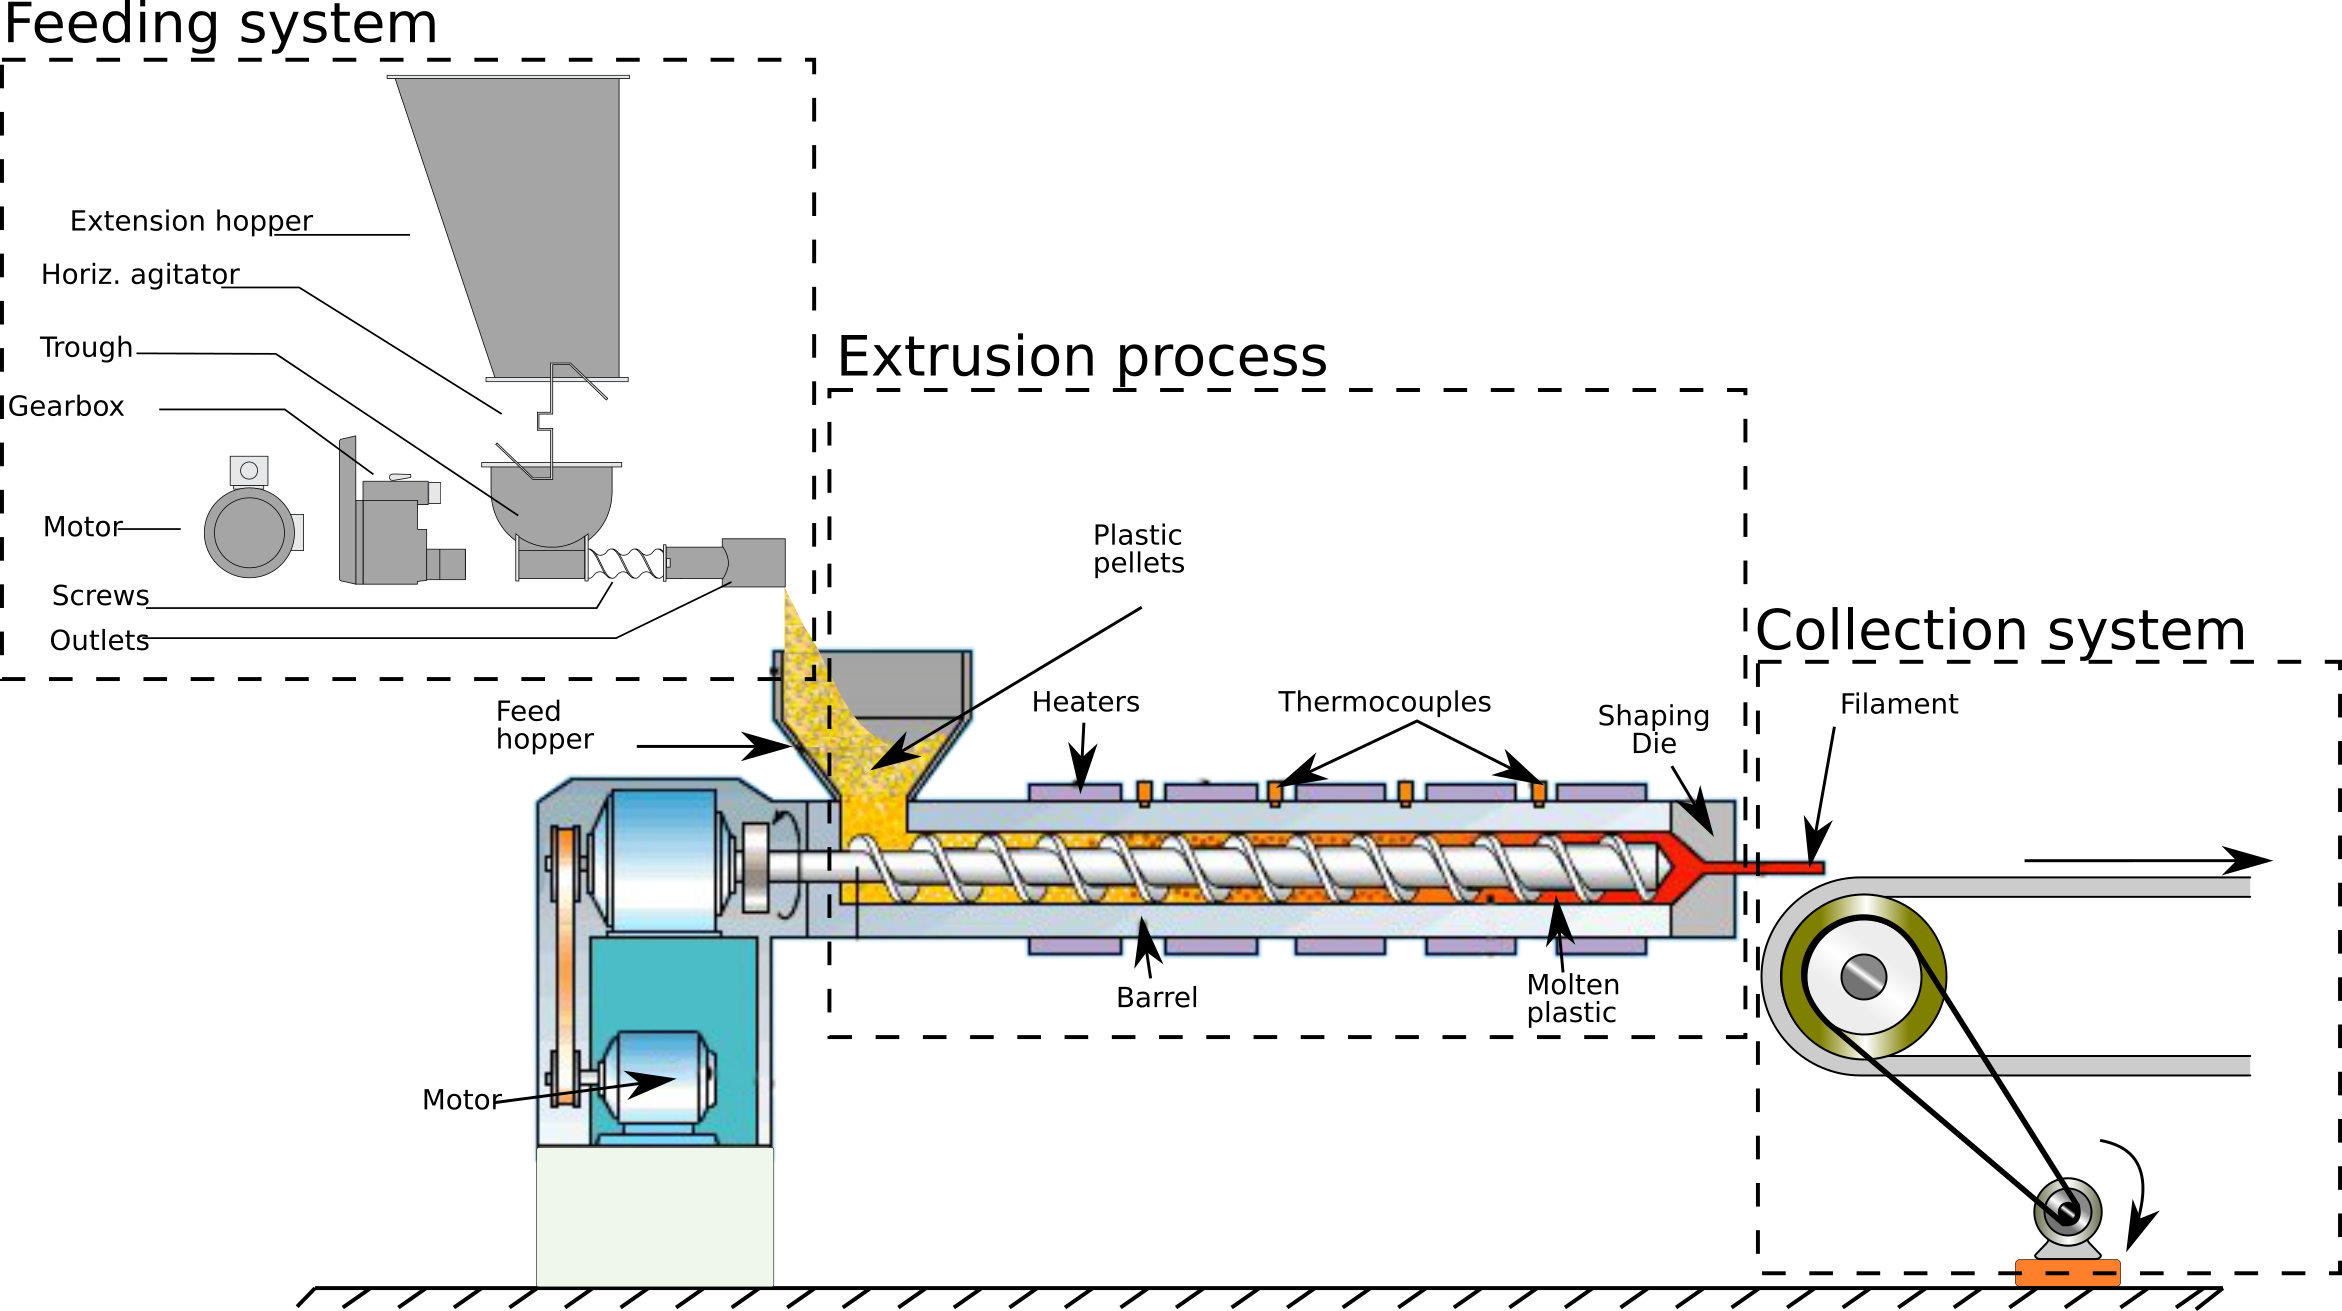
\includegraphics[width=1\linewidth]{https://raw.githubusercontent.com/fabbiocrux/Figures/main/Extrusion-process/Extrusion-process-00} 

}

\caption{Chaînes de recyclage pour évaluer la dégradation du matériau.}\label{fig:foldarap}
\end{figure}

Elles sont des imprimantes 3D représentatives de l'ensemble des machines
OS développées par la communauté RepRap, appelées Mondrian et FoldaRap
{[}126, 278, 279{]}. En effet, comme on peut le voir dans l'arbre
généalogique des imprimantes 3D open-source {[}16{]}. Ils sont une
variante de la machine RepRap avec une capacité de travail de
140×140×155(mm3) et 200×200×200(mm3) pour FoldaRap et Mondrian
respectivement. Le système d'extrusion peut être déplacé dans le plan
horizontal XY et le lit d'impression chauffé peut être déplacé dans la
direction verticale -Z. La resolution représentée est dans le plan X Y =
0.0125mm, Z = 0, 00025mm avec des tiges m5 et une précision:0.1mm. Le
lit d'impression chauffé est fait d'aluminium relié à une cellule
Peltier et il utilise une couche supérieure de kapton afin d'améliorer
l'adhérence de la pièce avec le lit d'impression.

La figure @ref(fig:parametros) montre les paramètres du processus à
prendre en compte pour la fabrication des échantillons imprimés. Ils
peuvent être définis comme suit :

\begin{figure}

{\centering 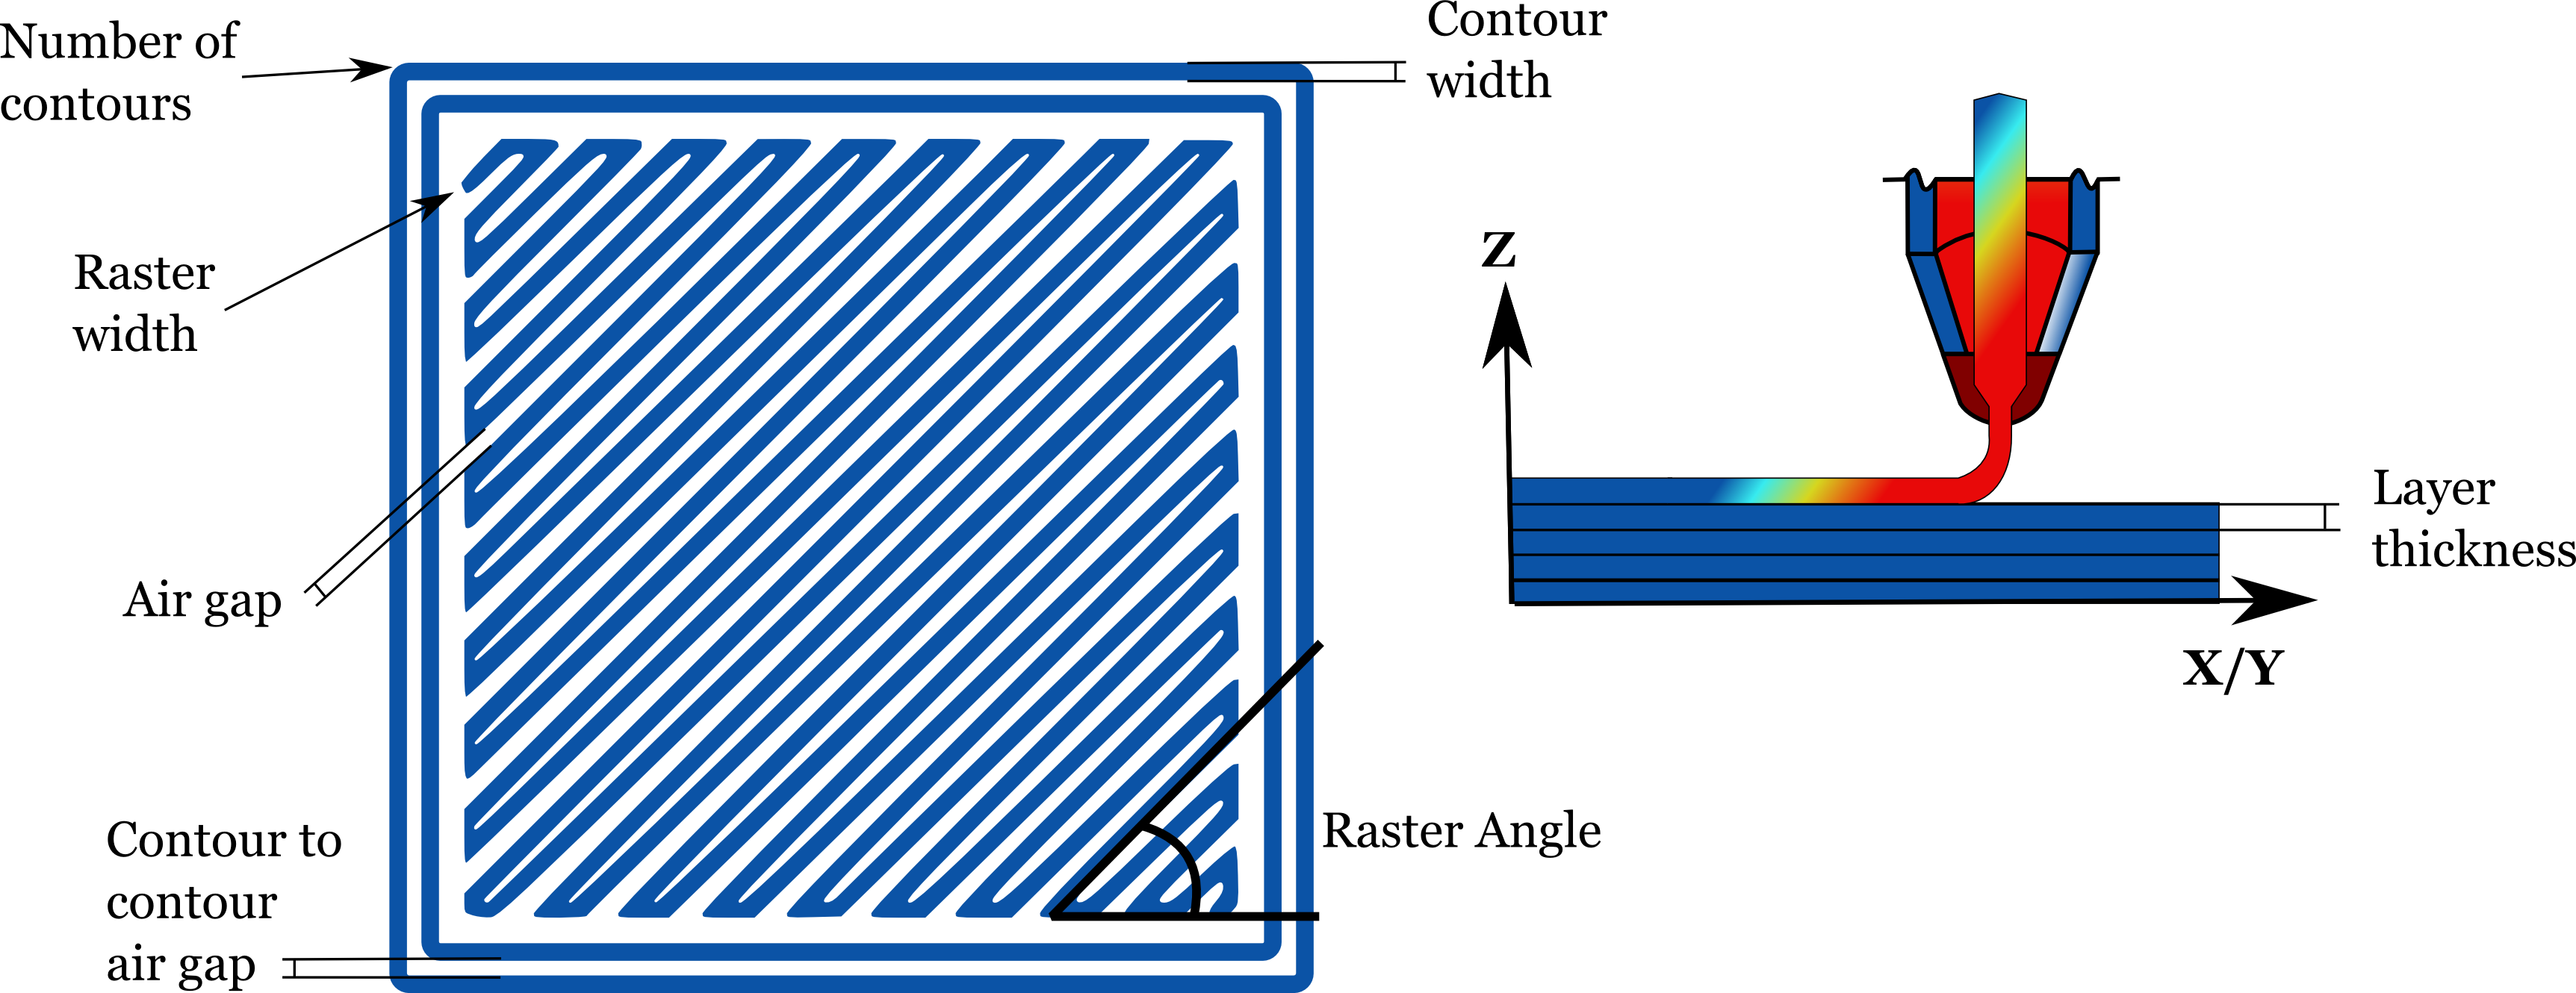
\includegraphics[width=1\linewidth]{https://raw.githubusercontent.com/fabbiocrux/Figures/main/AM/Process/Parametros} 

}

\caption{Chaînes de recyclage pour évaluer la dégradation du matériau.}\label{fig:parametros}
\end{figure}

\begin{itemize}
\tightlist
\item
  Direction de construction de la pièce : Il s'agit de l'inclinaison de
  la pièce dans une plate-forme de construction par rapport aux axes X,
  Y et Z. Les axes X et Y sont considérés comme parallèles à la
  plate-forme de construction. Les axes X et Y sont considérés comme
  parallèles à la plate-forme de construction. L'axe Z est considéré
  comme l'axe d'impression.
\item
  Épaisseur de la couche : Il s'agit de la hauteur de la couche déposée
  par la buse. Elle est généralement égale à la moitié de la largeur du
  cordon.
\item
  Angle de remplissage : Il s'agit de l'inclinaison des perles de
  filament déposées par rapport à l'axe x de la table d'usinage. Les
  configurations typiques sont 90/90 et 45/45.
\item
  Entrefer : C'est l'espace entre deux filaments adjacents de matériau
  sur la même couche. Une valeur nulle signifie que les trames se
  touchent. Une valeur positive signifie qu'il y a un espace. Une valeur
  négative signifie que les trames se chevauchent.
\item
  Nombre de contours : Définit le nombre de périmètres solides de
  l'objet.
\item
  Vitesse de la buse : C'est la vitesse de la buse de l'imprimante
  lorsqu'elle fabrique l'objet. (Vitesse des périmètres, petits
  périmètres, périmètres externes, remplissage - couches solides,
  supérieures, inférieures)
\end{itemize}

Du point de vue de la précision dimensionnelle, il y a eu des tentatives
pour caractériser la performance dimensionnelle des imprimantes 3D open
source {[}124-126, 230{]}. D'après les résultats obtenus dans le
chapitre 3, il a été constaté que, selon la norme internationale de
tolérance, le grade de ce type de machines pourrait être situé entre
IT14 et IT16. Une autre conclusion du chapitre 3 était que des
paramètres tels que l'épaisseur de la couche, la largeur de la trame et
la vitesse de déplacement de la buse peuvent avoir un impact sur la
précision de la machine {[}126{]}.

D'autre part, si l'on considère les propriétés mécaniques du matériau
dans la technologie de fabrication additive basée sur des systèmes de
bases extrudées, une conclusion importante de la littérature est qu'il
existe un comportement anisotrope. Cela signifie que le matériau est
dépendant de la direction. L'intégralité mécanique de la pièce imprimée
est directement liée à des facteurs tels que l'énergie
d'adhésion/cohésion entre les couches et les billes déposées, la
croissance de la zone de contact formée entre les billes adjacentes, la
dif- fusion moléculaire et la randomisation des chaînes de polymères à
travers l'interface, et un temps de résidence minimum à température
élevée afin d'assurer des niveaux adéquats de liaison diffusive
(\protect\hyperlink{ref-Agarwala1996}{Agarwala et al., 1996};
\protect\hyperlink{ref-AtifYardimci1996}{Atif Yardimci and Güçeri,
1996}; \protect\hyperlink{ref-Sun2008}{Sun et al., 2008};
\protect\hyperlink{ref-Yardimci1997}{Yardimci et al., 1997},). De plus,
l'histoire thermique des interfaces joue un rôle important dans la
détermination de la qualité du collage. Les cycles de chauffage et de
refroidissement inégaux dus à la nature inhérente du processus
d'impression entraînent une accumulation de contraintes dans la pièce
construite, ce qui est principalement responsable de la faiblesse du
collage et affecte donc la résistance. Pour cette raison, il existe une
dépendance des propriétés mécaniques par rapport aux parcours d'outils
et à l'orientation de la pièce. Par conséquent, les propriétés
mécaniques sont fonction des paramètres de fabrication car elles
affectent la méso-structure et la force de liaison entre les fibres
\protect\hyperlink{ref-Sood2010}{Sood et al.}
(\protect\hyperlink{ref-Sood2010}{2010})\}.

\hypertarget{etape-4---evaluation}{%
\subsection{Etape 4 - Evaluation}\label{etape-4---evaluation}}

La norme ISO 597 est utilisée afin de déterminer les propriétés de
traction du matériau recyclé. L'éprouvette utilisée est la norme ISO 527
1B. Le tableau 4.20 montre les mesures respectives de cette éprouvette.
Cette norme couvre les plastiques en tant que matériaux moulés, extrudés
et coulés, remplis et non remplis, les films et feuilles plastiques,
ainsi que les composites renforcés de fibres longues.

\hypertarget{etape-5---recyclage}{%
\subsection{Etape 5 - Recyclage}\label{etape-5---recyclage}}

La réduction de la taille des échantillons de chaque cycle de recyclage
est nécessaire afin de retraiter le matériau. Une broyeuse SM 300
Retsch® avec une plage de vitesse sélectionnable de 700 à 3 000 rpm a
été utilisée. La vitesse sélectionnée était de 700 rpm. La granulometrie
finale obtenue se situe dans une fourchette de 0,2 à 2 mm.

\hypertarget{resultats}{%
\section{Resultats}\label{resultats}}

A partir des quatre chaînes de recyclage, il est possible de comparer la
dégradation du matériau en utilisant un procédé traditionnel tels que
l'injection et le procédé d'impression 3D. La figure
@ref(fig:Comparation-mechanical-properties-Fr) présente le résultat de
notre démarche expérimentale.

\begin{center}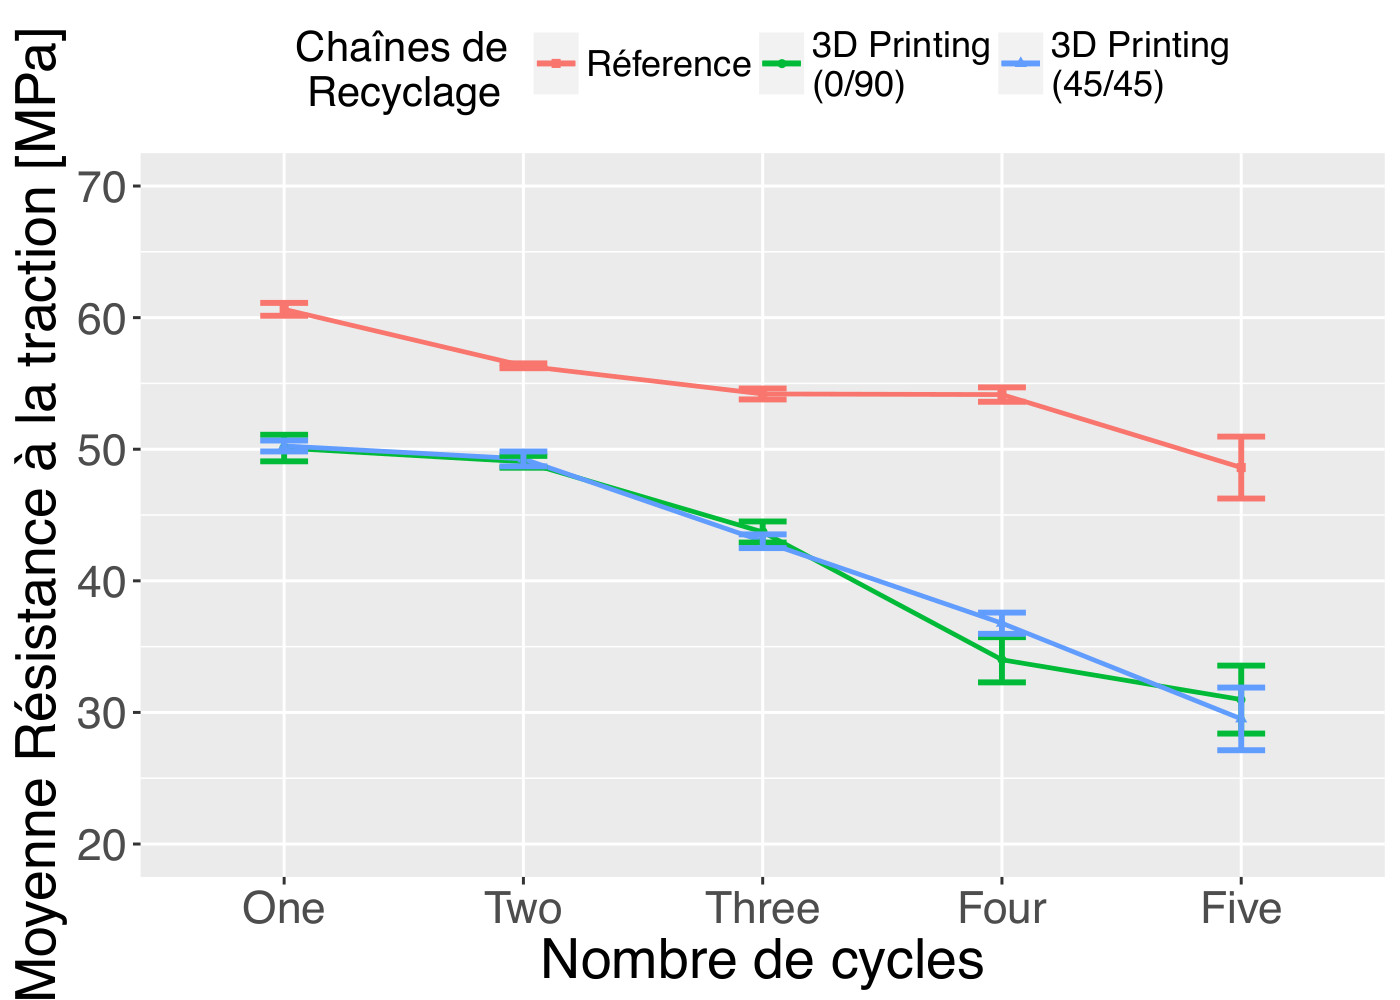
\includegraphics[width=0.48\linewidth]{https://raw.githubusercontent.com/fabbiocrux/Figures/main/Thesis/fr/Ref-3DP-Tensile-Strength} 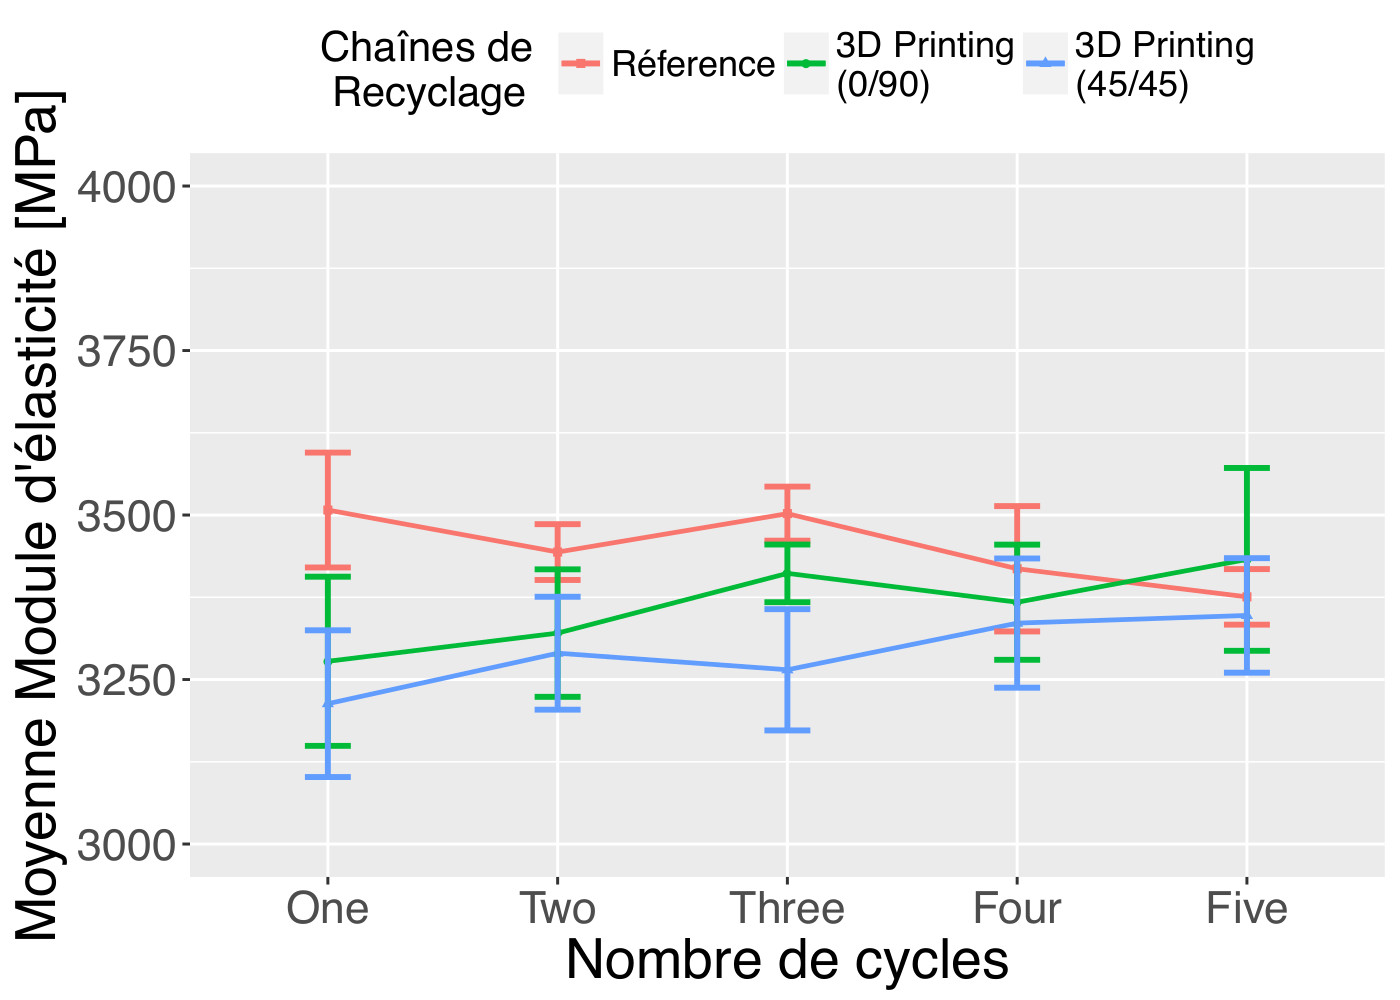
\includegraphics[width=0.48\linewidth]{https://raw.githubusercontent.com/fabbiocrux/Figures/main/Thesis/fr/Ref-3DP-Elastic-Modulus} 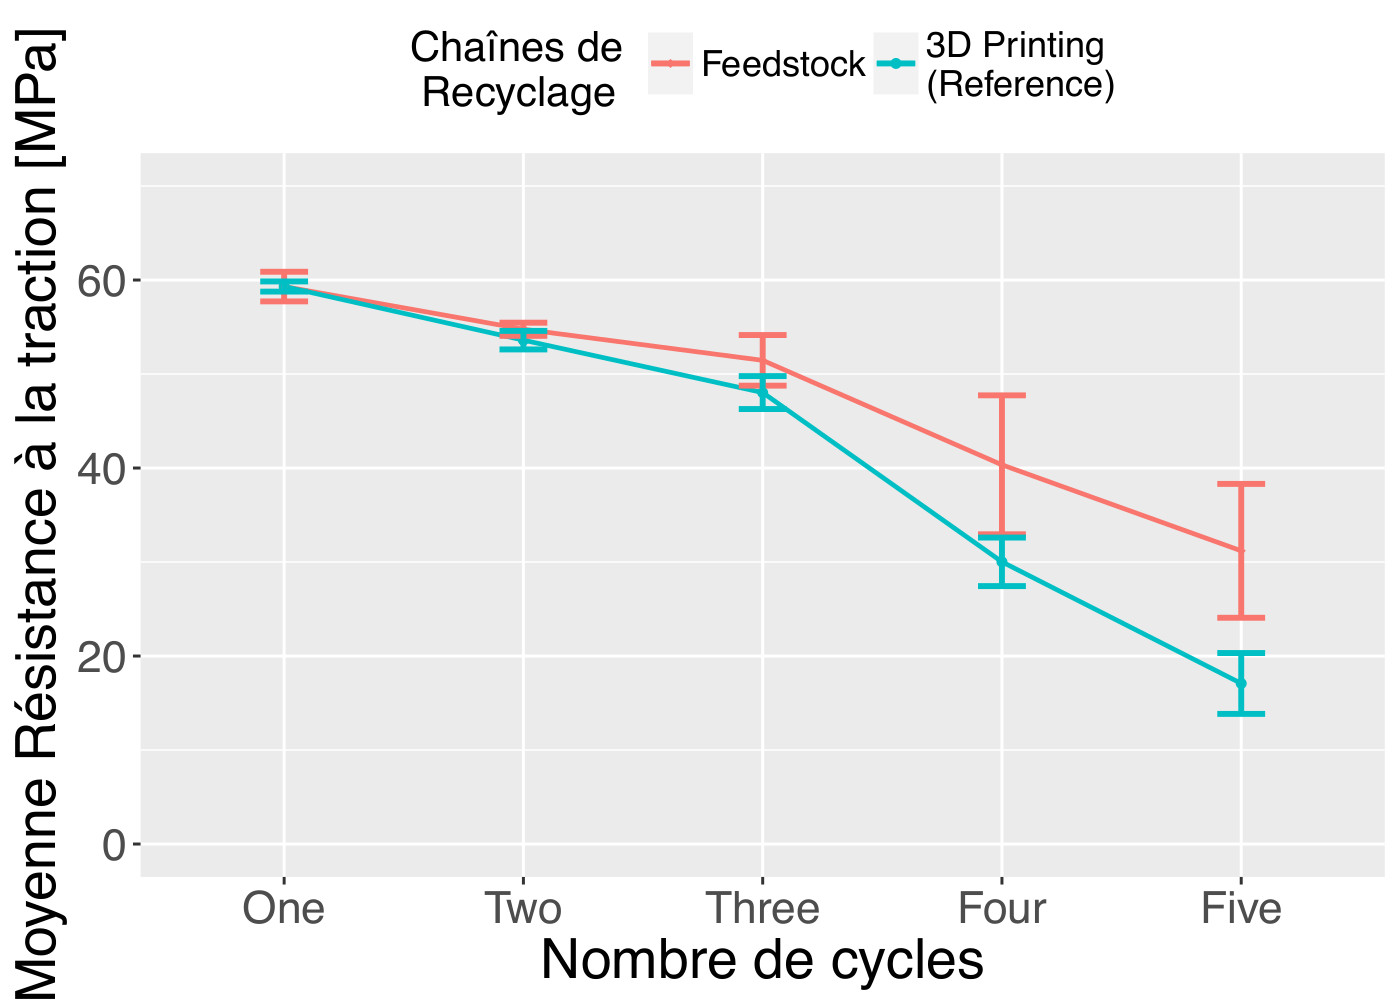
\includegraphics[width=0.48\linewidth]{https://raw.githubusercontent.com/fabbiocrux/Figures/main/Thesis/fr/Fed-3DP-Tensile-Strength} 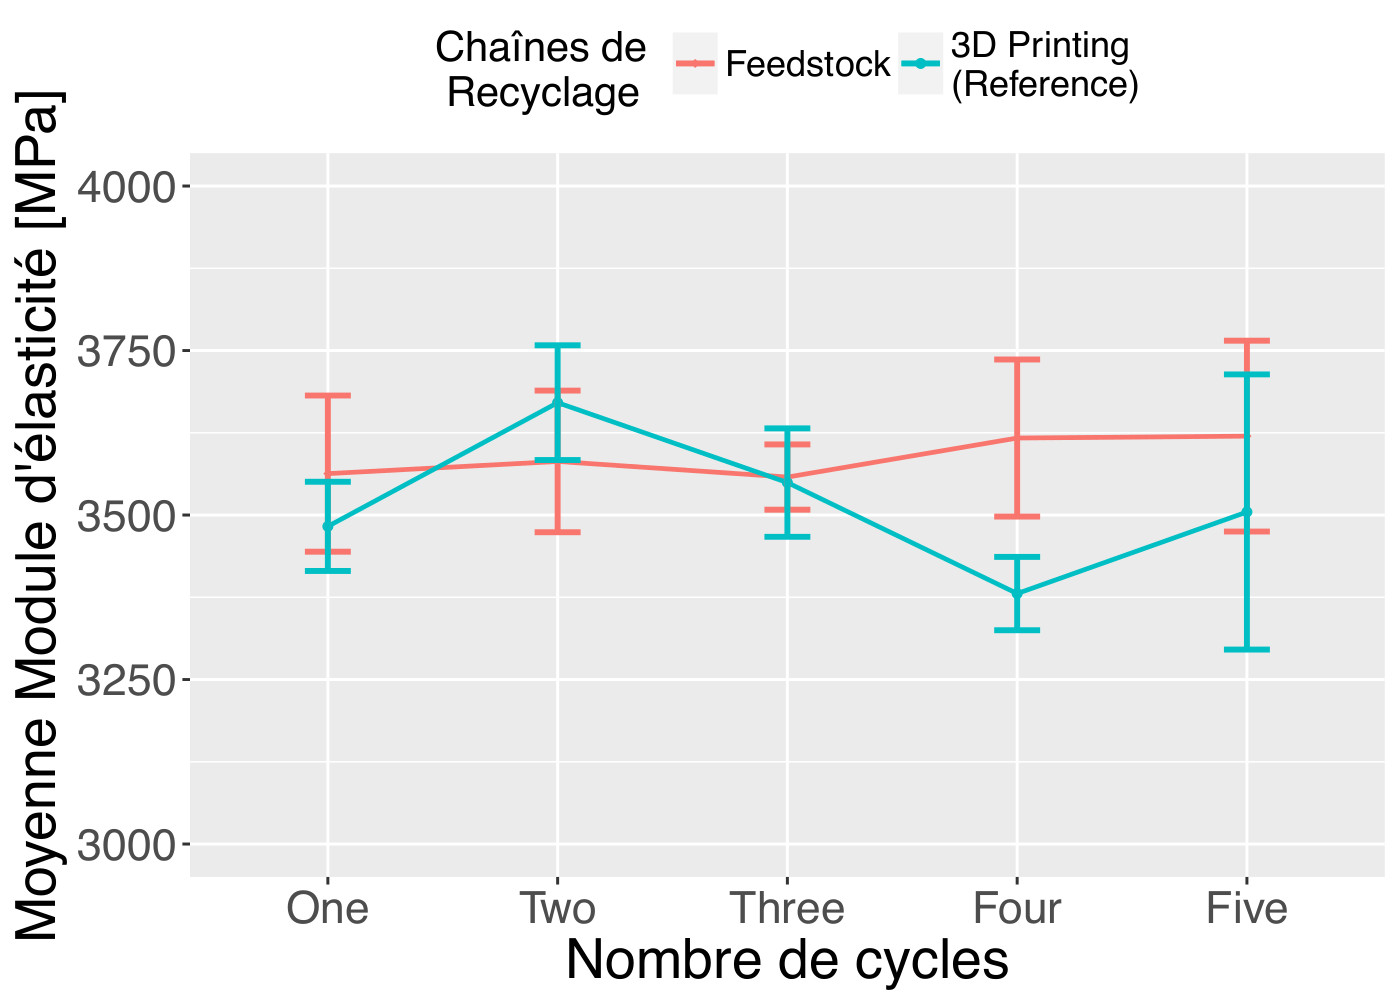
\includegraphics[width=0.48\linewidth]{https://raw.githubusercontent.com/fabbiocrux/Figures/main/Thesis/fr/Fed-3DP-Elastic-Modulus} \end{center}

Nous avons sélectionné 8 échantillons pour chaque chaîne de recyclage
afin d'avoir suffisamment de reproductibilité dans nos résultats. Dans
le cas de la chaîne \emph{3D Printing}, 16 échantillons ont été
sélectionnes 8 pour le remplissage \(0/90\) et 8 pour le cas de
\(45/45\). Une première observation de la comparaison est que dans tous
le cas, les échantillons injectés présentent des meilleure propriétés
que ceux imprimés tel qu'il est présenté dans la figure
@ref(fig:Comparation-mechanical-properties-Fr). La différence entre ces
deux procédés de fabrication est d'environ 10 \emph{MPa} dans le
première cycle, qui est en accord avec la littérature
(\protect\hyperlink{ref-Tymrak2014a}{Tymrak et al., 2014};
\protect\hyperlink{ref-Wittbrodt2015}{Wittbrodt and Pearce, 2015}).
Cependant, cette différence augmente jusqu'à environ 20 \emph{MPa} dans
le cinquième cycle.

Les résultats représentés dans la figure
@ref(fig:Comparation-mechanical-properties-Fr)B montrent que le module
élastique peut être considéré comme indépendant du processus de
recyclage et de fabrication. Il pourrait être considéré comme constant
pour les échantillons injectés (chaîne \emph{Reference}) dans une
intervalle de variation entre \(3300-3500\) \emph{MPa}. Pour le cas des
échantillons imprimés (\(45/45\) et \(0/90\) ), une faible augmentation
du module élastique est observée du premier au dernier cycle avec de
valeurs moyennes de \(3277.7\) à \(3432.6\) \emph{MPa} respectivement.

Une possible explication à cette augmentation du module d'élasticité
pour les échantillons imprimés, est qu'elle est associée au changement
de viscosité du matériau, conséquence du procédé de recyclage. Les
caractéristiques de la méso-structure et de la liaison fibre-fibre des
échantillons d'impression changeront aussi à mesure que le nombre de
cycles de recyclage augmente. Selon la littérature, certains défauts
internes qui affectent la qualité structurale des pièces imprimées sont
les vides, les pores et les vides sous-périmétriques dus à la forme
arrondie et oblongue du matériau déposé
(\protect\hyperlink{ref-Agarwala1996}{Agarwala et al., 1996};
\protect\hyperlink{ref-NTurner2014}{N. Turner et al., 2014}). Dans le
procédé d'impression, le matériau imprimé se propage dans une forme
oblongue dont la vitesse d'étalement et la forme finale dépendent de la
viscosité de la matière fondue et des énergies de surface relatives de
la trame déposé et de la surface sur laquelle elle est imprimée
(\protect\hyperlink{ref-NTurner2014}{N. Turner et al., 2014}).
Finalement, les propriétés mécaniques globales de la pièce dépendront de
la zone de contact entre les trames (et les couches) déposées, de la
taille des vides et des propriétés du matériau elles-mêmes.

Par conséquent, une hypothèse pour expliquer le comportement similaire
entre les chaînes de processus \emph{Reference} et \emph{3D Printing} en
termes de module élastique à la fin du cinquième cycle est qu'il y a une
réduction appréciable des défauts internes, provoquée par la diminution
de la viscosité du matériau, ce qui facilite l'homogénéisation des
couches déposées. Nous pouvons alors présumer, que la méso-structure
interne des échantillons imprimés pourrait être similaire à celle de
l'injection. Néanmoins, cette réduction de la viscosité est une
conséquence de la dégradation du matériau, entrainant l'un changement de
de propriétés de traction.

D'autre part, les figures
@ref(fig:Comparation-mechanical-properties-Fr)C et
@ref(fig:Comparation-mechanical-properties-Fr)D montrent les résultats
des propriétés mécaniques des chaînes de recyclage \emph{Feedstock} et
\emph{3D Printing (Réference)}. L'unique différence entre ces deux
chaînes est un processus d'impression 3D dans la dégradation du
matériau. Concernant le module d'élasticité, nous pouvons voir que cette
propriété reste virtuellement constante pendant le cycles. Nous pouvons
constater qu'il existe un effet de l'impression 3D sur le matériau. Il
est négligeable quand la matière est vierge, par contre, cette influence
augmente au fur et à mesure que le matériau est de plus en plus dégradé.
Il est important d'analyser ces résultats d'un point de vue chimique
afin de caractériser la dégradation au niveau microscopique.

les résultats spécifiques peuvent être résumés comme suit dans le
Tableau @ref(tab:table-summary):

\providecommand{\docline}[3]{\noalign{\global\setlength{\arrayrulewidth}{#1}}\arrayrulecolor[HTML]{#2}\cline{#3}}

\setlength{\tabcolsep}{2pt}

\renewcommand*{\arraystretch}{1.5}

\begin{longtable}[c]{|p{1.89in}|p{1.54in}|p{1.86in}|p{1.86in}|p{1.94in}|p{1.93in}}

\caption{Variation des propriétés mécaniques du PLA après cinq cycles de recyclage.}\\

\hhline{~~~~~~}

\multicolumn{1}{!{\color[HTML]{000000}\vrule width 0pt}>{\cellcolor[HTML]{CFCFCF}\raggedright}p{\dimexpr 1.89in+0\tabcolsep+0\arrayrulewidth}}{\fontsize{11}{11}\selectfont{\textcolor[HTML]{000000}{\textbf{Chaîne de Recyclage}}}} & \multicolumn{1}{!{\color[HTML]{000000}\vrule width 0pt}>{\cellcolor[HTML]{CFCFCF}\raggedright}p{\dimexpr 1.54in+0\tabcolsep+0\arrayrulewidth}}{\fontsize{11}{11}\selectfont{\textcolor[HTML]{000000}{\textbf{Module d'élasticité}}}} & \multicolumn{1}{!{\color[HTML]{000000}\vrule width 0pt}>{\cellcolor[HTML]{CFCFCF}\raggedright}p{\dimexpr 1.86in+0\tabcolsep+0\arrayrulewidth}}{\fontsize{11}{11}\selectfont{\textcolor[HTML]{000000}{\textbf{Résistance à la tension}}}} & \multicolumn{1}{!{\color[HTML]{000000}\vrule width 0pt}>{\cellcolor[HTML]{CFCFCF}\raggedright}p{\dimexpr 1.86in+0\tabcolsep+0\arrayrulewidth}}{\fontsize{11}{11}\selectfont{\textcolor[HTML]{000000}{\textbf{Résistance a la rupture}}}} & \multicolumn{1}{!{\color[HTML]{000000}\vrule width 0pt}>{\cellcolor[HTML]{CFCFCF}\raggedright}p{\dimexpr 1.94in+0\tabcolsep+0\arrayrulewidth}}{\fontsize{11}{11}\selectfont{\textcolor[HTML]{000000}{\textbf{Déformation à la tension}}}} & \multicolumn{1}{!{\color[HTML]{000000}\vrule width 0pt}>{\cellcolor[HTML]{CFCFCF}\raggedright}p{\dimexpr 1.93in+0\tabcolsep+0\arrayrulewidth}!{\color[HTML]{000000}\vrule width 0pt}}{\fontsize{11}{11}\selectfont{\textcolor[HTML]{000000}{\textbf{Déformation à la rupture}}}} \\



\endfirsthead

\hhline{~~~~~~}

\multicolumn{1}{!{\color[HTML]{000000}\vrule width 0pt}>{\cellcolor[HTML]{CFCFCF}\raggedright}p{\dimexpr 1.89in+0\tabcolsep+0\arrayrulewidth}}{\fontsize{11}{11}\selectfont{\textcolor[HTML]{000000}{\textbf{Chaîne de Recyclage}}}} & \multicolumn{1}{!{\color[HTML]{000000}\vrule width 0pt}>{\cellcolor[HTML]{CFCFCF}\raggedright}p{\dimexpr 1.54in+0\tabcolsep+0\arrayrulewidth}}{\fontsize{11}{11}\selectfont{\textcolor[HTML]{000000}{\textbf{Module d'élasticité}}}} & \multicolumn{1}{!{\color[HTML]{000000}\vrule width 0pt}>{\cellcolor[HTML]{CFCFCF}\raggedright}p{\dimexpr 1.86in+0\tabcolsep+0\arrayrulewidth}}{\fontsize{11}{11}\selectfont{\textcolor[HTML]{000000}{\textbf{Résistance à la tension}}}} & \multicolumn{1}{!{\color[HTML]{000000}\vrule width 0pt}>{\cellcolor[HTML]{CFCFCF}\raggedright}p{\dimexpr 1.86in+0\tabcolsep+0\arrayrulewidth}}{\fontsize{11}{11}\selectfont{\textcolor[HTML]{000000}{\textbf{Résistance a la rupture}}}} & \multicolumn{1}{!{\color[HTML]{000000}\vrule width 0pt}>{\cellcolor[HTML]{CFCFCF}\raggedright}p{\dimexpr 1.94in+0\tabcolsep+0\arrayrulewidth}}{\fontsize{11}{11}\selectfont{\textcolor[HTML]{000000}{\textbf{Déformation à la tension}}}} & \multicolumn{1}{!{\color[HTML]{000000}\vrule width 0pt}>{\cellcolor[HTML]{CFCFCF}\raggedright}p{\dimexpr 1.93in+0\tabcolsep+0\arrayrulewidth}!{\color[HTML]{000000}\vrule width 0pt}}{\fontsize{11}{11}\selectfont{\textcolor[HTML]{000000}{\textbf{Déformation à la rupture}}}} \\

\endhead



\multicolumn{1}{!{\color[HTML]{000000}\vrule width 0pt}>{\cellcolor[HTML]{EFEFEF}\raggedright}p{\dimexpr 1.89in+0\tabcolsep+0\arrayrulewidth}}{\fontsize{11}{11}\selectfont{\textcolor[HTML]{000000}{Référence}}} & \multicolumn{1}{!{\color[HTML]{000000}\vrule width 0pt}>{\cellcolor[HTML]{EFEFEF}\raggedright}p{\dimexpr 1.54in+0\tabcolsep+0\arrayrulewidth}}{\fontsize{11}{11}\selectfont{\textcolor[HTML]{000000}{-3.7\%}}} & \multicolumn{1}{!{\color[HTML]{000000}\vrule width 0pt}>{\cellcolor[HTML]{EFEFEF}\raggedright}p{\dimexpr 1.86in+0\tabcolsep+0\arrayrulewidth}}{\fontsize{11}{11}\selectfont{\textcolor[HTML]{000000}{-19.81\%}}} & \multicolumn{1}{!{\color[HTML]{000000}\vrule width 0pt}>{\cellcolor[HTML]{EFEFEF}\raggedright}p{\dimexpr 1.86in+0\tabcolsep+0\arrayrulewidth}}{\fontsize{11}{11}\selectfont{\textcolor[HTML]{000000}{-15.95\%}}} & \multicolumn{1}{!{\color[HTML]{000000}\vrule width 0pt}>{\cellcolor[HTML]{EFEFEF}\raggedright}p{\dimexpr 1.94in+0\tabcolsep+0\arrayrulewidth}}{\fontsize{11}{11}\selectfont{\textcolor[HTML]{000000}{-27.31\%}}} & \multicolumn{1}{!{\color[HTML]{000000}\vrule width 0pt}>{\cellcolor[HTML]{EFEFEF}\raggedright}p{\dimexpr 1.93in+0\tabcolsep+0\arrayrulewidth}!{\color[HTML]{000000}\vrule width 0pt}}{\fontsize{11}{11}\selectfont{\textcolor[HTML]{000000}{-40.65\%}}} \\





\multicolumn{1}{!{\color[HTML]{000000}\vrule width 0pt}>{\raggedright}p{\dimexpr 1.89in+0\tabcolsep+0\arrayrulewidth}}{\fontsize{11}{11}\selectfont{\textcolor[HTML]{000000}{3D Printing (0/90)}}} & \multicolumn{1}{!{\color[HTML]{000000}\vrule width 0pt}>{\raggedright}p{\dimexpr 1.54in+0\tabcolsep+0\arrayrulewidth}}{\fontsize{11}{11}\selectfont{\textcolor[HTML]{000000}{+4.1\%}}} & \multicolumn{1}{!{\color[HTML]{000000}\vrule width 0pt}>{\raggedright}p{\dimexpr 1.86in+0\tabcolsep+0\arrayrulewidth}}{\fontsize{11}{11}\selectfont{\textcolor[HTML]{000000}{-38.15\%}}} & \multicolumn{1}{!{\color[HTML]{000000}\vrule width 0pt}>{\raggedright}p{\dimexpr 1.86in+0\tabcolsep+0\arrayrulewidth}}{\fontsize{11}{11}\selectfont{\textcolor[HTML]{000000}{-39.29\%}}} & \multicolumn{1}{!{\color[HTML]{000000}\vrule width 0pt}>{\raggedright}p{\dimexpr 1.94in+0\tabcolsep+0\arrayrulewidth}}{\fontsize{11}{11}\selectfont{\textcolor[HTML]{000000}{-52.20\%}}} & \multicolumn{1}{!{\color[HTML]{000000}\vrule width 0pt}>{\raggedright}p{\dimexpr 1.93in+0\tabcolsep+0\arrayrulewidth}!{\color[HTML]{000000}\vrule width 0pt}}{\fontsize{11}{11}\selectfont{\textcolor[HTML]{000000}{-57.43\%}}} \\





\multicolumn{1}{!{\color[HTML]{000000}\vrule width 0pt}>{\cellcolor[HTML]{EFEFEF}\raggedright}p{\dimexpr 1.89in+0\tabcolsep+0\arrayrulewidth}}{\fontsize{11}{11}\selectfont{\textcolor[HTML]{000000}{3D Printing (45/45)}}} & \multicolumn{1}{!{\color[HTML]{000000}\vrule width 0pt}>{\cellcolor[HTML]{EFEFEF}\raggedright}p{\dimexpr 1.54in+0\tabcolsep+0\arrayrulewidth}}{\fontsize{11}{11}\selectfont{\textcolor[HTML]{000000}{+4.7\%}}} & \multicolumn{1}{!{\color[HTML]{000000}\vrule width 0pt}>{\cellcolor[HTML]{EFEFEF}\raggedright}p{\dimexpr 1.86in+0\tabcolsep+0\arrayrulewidth}}{\fontsize{11}{11}\selectfont{\textcolor[HTML]{000000}{-41.27\%}}} & \multicolumn{1}{!{\color[HTML]{000000}\vrule width 0pt}>{\cellcolor[HTML]{EFEFEF}\raggedright}p{\dimexpr 1.86in+0\tabcolsep+0\arrayrulewidth}}{\fontsize{11}{11}\selectfont{\textcolor[HTML]{000000}{-40.08\%}}} & \multicolumn{1}{!{\color[HTML]{000000}\vrule width 0pt}>{\cellcolor[HTML]{EFEFEF}\raggedright}p{\dimexpr 1.94in+0\tabcolsep+0\arrayrulewidth}}{\fontsize{11}{11}\selectfont{\textcolor[HTML]{000000}{-53.08\%}}} & \multicolumn{1}{!{\color[HTML]{000000}\vrule width 0pt}>{\cellcolor[HTML]{EFEFEF}\raggedright}p{\dimexpr 1.93in+0\tabcolsep+0\arrayrulewidth}!{\color[HTML]{000000}\vrule width 0pt}}{\fontsize{11}{11}\selectfont{\textcolor[HTML]{000000}{-56.53\%}}} \\





\multicolumn{1}{!{\color[HTML]{000000}\vrule width 0pt}>{\raggedright}p{\dimexpr 1.89in+0\tabcolsep+0\arrayrulewidth}}{\fontsize{11}{11}\selectfont{\textcolor[HTML]{000000}{Feedstock}}} & \multicolumn{1}{!{\color[HTML]{000000}\vrule width 0pt}>{\raggedright}p{\dimexpr 1.54in+0\tabcolsep+0\arrayrulewidth}}{\fontsize{11}{11}\selectfont{\textcolor[HTML]{000000}{Constant}}} & \multicolumn{1}{!{\color[HTML]{000000}\vrule width 0pt}>{\raggedright}p{\dimexpr 1.86in+0\tabcolsep+0\arrayrulewidth}}{\fontsize{11}{11}\selectfont{\textcolor[HTML]{000000}{-47.56\%}}} & \multicolumn{1}{!{\color[HTML]{000000}\vrule width 0pt}>{\raggedright}p{\dimexpr 1.86in+0\tabcolsep+0\arrayrulewidth}}{\fontsize{11}{11}\selectfont{\textcolor[HTML]{000000}{-42.52\%}}} & \multicolumn{1}{!{\color[HTML]{000000}\vrule width 0pt}>{\raggedright}p{\dimexpr 1.94in+0\tabcolsep+0\arrayrulewidth}}{\fontsize{11}{11}\selectfont{\textcolor[HTML]{000000}{-58.57\%}}} & \multicolumn{1}{!{\color[HTML]{000000}\vrule width 0pt}>{\raggedright}p{\dimexpr 1.93in+0\tabcolsep+0\arrayrulewidth}!{\color[HTML]{000000}\vrule width 0pt}}{\fontsize{11}{11}\selectfont{\textcolor[HTML]{000000}{-70.84\%}}} \\





\multicolumn{1}{!{\color[HTML]{000000}\vrule width 0pt}>{\cellcolor[HTML]{EFEFEF}\raggedright}p{\dimexpr 1.89in+0\tabcolsep+0\arrayrulewidth}}{\fontsize{11}{11}\selectfont{\textcolor[HTML]{000000}{3D Printing (Reference)}}} & \multicolumn{1}{!{\color[HTML]{000000}\vrule width 0pt}>{\cellcolor[HTML]{EFEFEF}\raggedright}p{\dimexpr 1.54in+0\tabcolsep+0\arrayrulewidth}}{\fontsize{11}{11}\selectfont{\textcolor[HTML]{000000}{Constant}}} & \multicolumn{1}{!{\color[HTML]{000000}\vrule width 0pt}>{\cellcolor[HTML]{EFEFEF}\raggedright}p{\dimexpr 1.86in+0\tabcolsep+0\arrayrulewidth}}{\fontsize{11}{11}\selectfont{\textcolor[HTML]{000000}{-71.34\%}}} & \multicolumn{1}{!{\color[HTML]{000000}\vrule width 0pt}>{\cellcolor[HTML]{EFEFEF}\raggedright}p{\dimexpr 1.86in+0\tabcolsep+0\arrayrulewidth}}{\fontsize{11}{11}\selectfont{\textcolor[HTML]{000000}{-72.58\%}}} & \multicolumn{1}{!{\color[HTML]{000000}\vrule width 0pt}>{\cellcolor[HTML]{EFEFEF}\raggedright}p{\dimexpr 1.94in+0\tabcolsep+0\arrayrulewidth}}{\fontsize{11}{11}\selectfont{\textcolor[HTML]{000000}{-78.93\%}}} & \multicolumn{1}{!{\color[HTML]{000000}\vrule width 0pt}>{\cellcolor[HTML]{EFEFEF}\raggedright}p{\dimexpr 1.93in+0\tabcolsep+0\arrayrulewidth}!{\color[HTML]{000000}\vrule width 0pt}}{\fontsize{11}{11}\selectfont{\textcolor[HTML]{000000}{-86.49\%}}} \\



\end{longtable}

Le tableau @ref(tab:table-demarche) montre un résumé des éléments les
plus importants qui ont été considérés lors de l'application de la
méthodologie.

\providecommand{\docline}[3]{\noalign{\global\setlength{\arrayrulewidth}{#1}}\arrayrulecolor[HTML]{#2}\cline{#3}}

\setlength{\tabcolsep}{2pt}

\renewcommand*{\arraystretch}{1.5}

\begin{longtable}[c]{|p{0.50in}|p{1.89in}|p{2.48in}|p{2.89in}}

\caption{Application de la méthodologie au cas du recyclage du PLA pour l’impression 3D.}\\

\hhline{~~~~}

\multicolumn{1}{!{\color[HTML]{000000}\vrule width 0pt}>{\cellcolor[HTML]{CFCFCF}\raggedleft}p{\dimexpr 0.5in+0\tabcolsep+0\arrayrulewidth}}{\fontsize{11}{11}\selectfont{\textcolor[HTML]{000000}{\textbf{X1}}}} & \multicolumn{1}{!{\color[HTML]{000000}\vrule width 0pt}>{\cellcolor[HTML]{CFCFCF}\raggedright}p{\dimexpr 1.89in+0\tabcolsep+0\arrayrulewidth}}{\fontsize{11}{11}\selectfont{\textcolor[HTML]{000000}{\textbf{Étape}}}} & \multicolumn{1}{!{\color[HTML]{000000}\vrule width 0pt}>{\cellcolor[HTML]{CFCFCF}\raggedright}p{\dimexpr 2.48in+0\tabcolsep+0\arrayrulewidth}}{\fontsize{11}{11}\selectfont{\textcolor[HTML]{000000}{\textbf{Éléments à Définir}}}} & \multicolumn{1}{!{\color[HTML]{000000}\vrule width 0pt}>{\cellcolor[HTML]{CFCFCF}\raggedright}p{\dimexpr 2.89in+0\tabcolsep+0\arrayrulewidth}!{\color[HTML]{000000}\vrule width 0pt}}{\fontsize{11}{11}\selectfont{\textcolor[HTML]{000000}{\textbf{Notre cas expérimental}}}} \\



\endfirsthead

\hhline{~~~~}

\multicolumn{1}{!{\color[HTML]{000000}\vrule width 0pt}>{\cellcolor[HTML]{CFCFCF}\raggedleft}p{\dimexpr 0.5in+0\tabcolsep+0\arrayrulewidth}}{\fontsize{11}{11}\selectfont{\textcolor[HTML]{000000}{\textbf{X1}}}} & \multicolumn{1}{!{\color[HTML]{000000}\vrule width 0pt}>{\cellcolor[HTML]{CFCFCF}\raggedright}p{\dimexpr 1.89in+0\tabcolsep+0\arrayrulewidth}}{\fontsize{11}{11}\selectfont{\textcolor[HTML]{000000}{\textbf{Étape}}}} & \multicolumn{1}{!{\color[HTML]{000000}\vrule width 0pt}>{\cellcolor[HTML]{CFCFCF}\raggedright}p{\dimexpr 2.48in+0\tabcolsep+0\arrayrulewidth}}{\fontsize{11}{11}\selectfont{\textcolor[HTML]{000000}{\textbf{Éléments à Définir}}}} & \multicolumn{1}{!{\color[HTML]{000000}\vrule width 0pt}>{\cellcolor[HTML]{CFCFCF}\raggedright}p{\dimexpr 2.89in+0\tabcolsep+0\arrayrulewidth}!{\color[HTML]{000000}\vrule width 0pt}}{\fontsize{11}{11}\selectfont{\textcolor[HTML]{000000}{\textbf{Notre cas expérimental}}}} \\

\endhead



\multicolumn{1}{!{\color[HTML]{000000}\vrule width 0pt}>{\cellcolor[HTML]{EFEFEF}\raggedleft}p{\dimexpr 0.5in+0\tabcolsep+0\arrayrulewidth}}{\fontsize{11}{11}\selectfont{\textcolor[HTML]{000000}{1.0}}} & \multicolumn{1}{!{\color[HTML]{000000}\vrule width 0pt}>{\cellcolor[HTML]{EFEFEF}\raggedright}p{\dimexpr 1.89in+0\tabcolsep+0\arrayrulewidth}}{\fontsize{11}{11}\selectfont{\textcolor[HTML]{000000}{Définition du matériau}}} & \multicolumn{1}{!{\color[HTML]{000000}\vrule width 0pt}>{\cellcolor[HTML]{EFEFEF}\raggedright}p{\dimexpr 2.48in+0\tabcolsep+0\arrayrulewidth}}{\fontsize{11}{11}\selectfont{\textcolor[HTML]{000000}{}}} & \multicolumn{1}{!{\color[HTML]{000000}\vrule width 0pt}>{\cellcolor[HTML]{EFEFEF}\raggedright}p{\dimexpr 2.89in+0\tabcolsep+0\arrayrulewidth}!{\color[HTML]{000000}\vrule width 0pt}}{\fontsize{11}{11}\selectfont{\textcolor[HTML]{000000}{Acide Polylactique (PLA)}}} \\





\multicolumn{1}{!{\color[HTML]{000000}\vrule width 0pt}>{\raggedleft}p{\dimexpr 0.5in+0\tabcolsep+0\arrayrulewidth}}{\fontsize{11}{11}\selectfont{\textcolor[HTML]{000000}{2.1}}} & \multicolumn{1}{!{\color[HTML]{000000}\vrule width 0pt}>{\raggedright}p{\dimexpr 1.89in+0\tabcolsep+0\arrayrulewidth}}{\fontsize{11}{11}\selectfont{\textcolor[HTML]{000000}{Procédés de Référence}}} & \multicolumn{1}{!{\color[HTML]{000000}\vrule width 0pt}>{\raggedright}p{\dimexpr 2.48in+0\tabcolsep+0\arrayrulewidth}}{\fontsize{11}{11}\selectfont{\textcolor[HTML]{000000}{Chaines de recyclage}}} & \multicolumn{1}{!{\color[HTML]{000000}\vrule width 0pt}>{\raggedright}p{\dimexpr 2.89in+0\tabcolsep+0\arrayrulewidth}!{\color[HTML]{000000}\vrule width 0pt}}{\fontsize{11}{11}\selectfont{\textcolor[HTML]{000000}{Quatre chaînes de recyclage}}} \\





\multicolumn{1}{!{\color[HTML]{000000}\vrule width 0pt}>{\cellcolor[HTML]{EFEFEF}\raggedleft}p{\dimexpr 0.5in+0\tabcolsep+0\arrayrulewidth}}{\fontsize{11}{11}\selectfont{\textcolor[HTML]{000000}{2.1}}} & \multicolumn{1}{!{\color[HTML]{000000}\vrule width 0pt}>{\cellcolor[HTML]{EFEFEF}\raggedright}p{\dimexpr 1.89in+0\tabcolsep+0\arrayrulewidth}}{\fontsize{11}{11}\selectfont{\textcolor[HTML]{000000}{Procédés de Référence}}} & \multicolumn{1}{!{\color[HTML]{000000}\vrule width 0pt}>{\cellcolor[HTML]{EFEFEF}\raggedright}p{\dimexpr 2.48in+0\tabcolsep+0\arrayrulewidth}}{\fontsize{11}{11}\selectfont{\textcolor[HTML]{000000}{Propriété à évaluer}}} & \multicolumn{1}{!{\color[HTML]{000000}\vrule width 0pt}>{\cellcolor[HTML]{EFEFEF}\raggedright}p{\dimexpr 2.89in+0\tabcolsep+0\arrayrulewidth}!{\color[HTML]{000000}\vrule width 0pt}}{\fontsize{11}{11}\selectfont{\textcolor[HTML]{000000}{Propriétes mécaniques}}} \\





\multicolumn{1}{!{\color[HTML]{000000}\vrule width 0pt}>{\raggedleft}p{\dimexpr 0.5in+0\tabcolsep+0\arrayrulewidth}}{\fontsize{11}{11}\selectfont{\textcolor[HTML]{000000}{2.2}}} & \multicolumn{1}{!{\color[HTML]{000000}\vrule width 0pt}>{\raggedright}p{\dimexpr 1.89in+0\tabcolsep+0\arrayrulewidth}}{\fontsize{11}{11}\selectfont{\textcolor[HTML]{000000}{Matière première}}} & \multicolumn{1}{!{\color[HTML]{000000}\vrule width 0pt}>{\raggedright}p{\dimexpr 2.48in+0\tabcolsep+0\arrayrulewidth}}{\fontsize{11}{11}\selectfont{\textcolor[HTML]{000000}{Procédé de fabrication}}} & \multicolumn{1}{!{\color[HTML]{000000}\vrule width 0pt}>{\raggedright}p{\dimexpr 2.89in+0\tabcolsep+0\arrayrulewidth}!{\color[HTML]{000000}\vrule width 0pt}}{\fontsize{11}{11}\selectfont{\textcolor[HTML]{000000}{Extrusion}}} \\





\multicolumn{1}{!{\color[HTML]{000000}\vrule width 0pt}>{\cellcolor[HTML]{EFEFEF}\raggedleft}p{\dimexpr 0.5in+0\tabcolsep+0\arrayrulewidth}}{\fontsize{11}{11}\selectfont{\textcolor[HTML]{000000}{2.2}}} & \multicolumn{1}{!{\color[HTML]{000000}\vrule width 0pt}>{\cellcolor[HTML]{EFEFEF}\raggedright}p{\dimexpr 1.89in+0\tabcolsep+0\arrayrulewidth}}{\fontsize{11}{11}\selectfont{\textcolor[HTML]{000000}{pour l'Impression 3D}}} & \multicolumn{1}{!{\color[HTML]{000000}\vrule width 0pt}>{\cellcolor[HTML]{EFEFEF}\raggedright}p{\dimexpr 2.48in+0\tabcolsep+0\arrayrulewidth}}{\fontsize{11}{11}\selectfont{\textcolor[HTML]{000000}{Paramètre de Qualité}}} & \multicolumn{1}{!{\color[HTML]{000000}\vrule width 0pt}>{\cellcolor[HTML]{EFEFEF}\raggedright}p{\dimexpr 2.89in+0\tabcolsep+0\arrayrulewidth}!{\color[HTML]{000000}\vrule width 0pt}}{\fontsize{11}{11}\selectfont{\textcolor[HTML]{000000}{Diamètre du Filament}}} \\





\multicolumn{1}{!{\color[HTML]{000000}\vrule width 0pt}>{\raggedleft}p{\dimexpr 0.5in+0\tabcolsep+0\arrayrulewidth}}{\fontsize{11}{11}\selectfont{\textcolor[HTML]{000000}{3.1}}} & \multicolumn{1}{!{\color[HTML]{000000}\vrule width 0pt}>{\raggedright}p{\dimexpr 1.89in+0\tabcolsep+0\arrayrulewidth}}{\fontsize{11}{11}\selectfont{\textcolor[HTML]{000000}{Fabrication}}} & \multicolumn{1}{!{\color[HTML]{000000}\vrule width 0pt}>{\raggedright}p{\dimexpr 2.48in+0\tabcolsep+0\arrayrulewidth}}{\fontsize{11}{11}\selectfont{\textcolor[HTML]{000000}{Normes}}} & \multicolumn{1}{!{\color[HTML]{000000}\vrule width 0pt}>{\raggedright}p{\dimexpr 2.89in+0\tabcolsep+0\arrayrulewidth}!{\color[HTML]{000000}\vrule width 0pt}}{\fontsize{11}{11}\selectfont{\textcolor[HTML]{000000}{ISO 527-1B}}} \\





\multicolumn{1}{!{\color[HTML]{000000}\vrule width 0pt}>{\cellcolor[HTML]{EFEFEF}\raggedleft}p{\dimexpr 0.5in+0\tabcolsep+0\arrayrulewidth}}{\fontsize{11}{11}\selectfont{\textcolor[HTML]{000000}{3.1}}} & \multicolumn{1}{!{\color[HTML]{000000}\vrule width 0pt}>{\cellcolor[HTML]{EFEFEF}\raggedright}p{\dimexpr 1.89in+0\tabcolsep+0\arrayrulewidth}}{\fontsize{11}{11}\selectfont{\textcolor[HTML]{000000}{Standard}}} & \multicolumn{1}{!{\color[HTML]{000000}\vrule width 0pt}>{\cellcolor[HTML]{EFEFEF}\raggedright}p{\dimexpr 2.48in+0\tabcolsep+0\arrayrulewidth}}{\fontsize{11}{11}\selectfont{\textcolor[HTML]{000000}{Internationaux}}} & \multicolumn{1}{!{\color[HTML]{000000}\vrule width 0pt}>{\cellcolor[HTML]{EFEFEF}\raggedright}p{\dimexpr 2.89in+0\tabcolsep+0\arrayrulewidth}!{\color[HTML]{000000}\vrule width 0pt}}{\fontsize{11}{11}\selectfont{\textcolor[HTML]{000000}{(Propriétés Mécaniques)}}} \\





\multicolumn{1}{!{\color[HTML]{000000}\vrule width 0pt}>{\raggedleft}p{\dimexpr 0.5in+0\tabcolsep+0\arrayrulewidth}}{\fontsize{11}{11}\selectfont{\textcolor[HTML]{000000}{3.2}}} & \multicolumn{1}{!{\color[HTML]{000000}\vrule width 0pt}>{\raggedright}p{\dimexpr 1.89in+0\tabcolsep+0\arrayrulewidth}}{\fontsize{11}{11}\selectfont{\textcolor[HTML]{000000}{Fabrication}}} & \multicolumn{1}{!{\color[HTML]{000000}\vrule width 0pt}>{\raggedright}p{\dimexpr 2.48in+0\tabcolsep+0\arrayrulewidth}}{\fontsize{11}{11}\selectfont{\textcolor[HTML]{000000}{Caractérisation des Imprimantes}}} & \multicolumn{1}{!{\color[HTML]{000000}\vrule width 0pt}>{\raggedright}p{\dimexpr 2.89in+0\tabcolsep+0\arrayrulewidth}!{\color[HTML]{000000}\vrule width 0pt}}{\fontsize{11}{11}\selectfont{\textcolor[HTML]{000000}{FoldaRap}}} \\





\multicolumn{1}{!{\color[HTML]{000000}\vrule width 0pt}>{\cellcolor[HTML]{EFEFEF}\raggedleft}p{\dimexpr 0.5in+0\tabcolsep+0\arrayrulewidth}}{\fontsize{11}{11}\selectfont{\textcolor[HTML]{000000}{3.2}}} & \multicolumn{1}{!{\color[HTML]{000000}\vrule width 0pt}>{\cellcolor[HTML]{EFEFEF}\raggedright}p{\dimexpr 1.89in+0\tabcolsep+0\arrayrulewidth}}{\fontsize{11}{11}\selectfont{\textcolor[HTML]{000000}{Impression 3D}}} & \multicolumn{1}{!{\color[HTML]{000000}\vrule width 0pt}>{\cellcolor[HTML]{EFEFEF}\raggedright}p{\dimexpr 2.48in+0\tabcolsep+0\arrayrulewidth}}{\fontsize{11}{11}\selectfont{\textcolor[HTML]{000000}{Paramètres}}} & \multicolumn{1}{!{\color[HTML]{000000}\vrule width 0pt}>{\cellcolor[HTML]{EFEFEF}\raggedright}p{\dimexpr 2.89in+0\tabcolsep+0\arrayrulewidth}!{\color[HTML]{000000}\vrule width 0pt}}{\fontsize{11}{11}\selectfont{\textcolor[HTML]{000000}{Deux type d'éprouvettes (0/90 - 45/45)}}} \\





\multicolumn{1}{!{\color[HTML]{000000}\vrule width 0pt}>{\raggedleft}p{\dimexpr 0.5in+0\tabcolsep+0\arrayrulewidth}}{\fontsize{11}{11}\selectfont{\textcolor[HTML]{000000}{4.0}}} & \multicolumn{1}{!{\color[HTML]{000000}\vrule width 0pt}>{\raggedright}p{\dimexpr 1.89in+0\tabcolsep+0\arrayrulewidth}}{\fontsize{11}{11}\selectfont{\textcolor[HTML]{000000}{Evaluation}}} & \multicolumn{1}{!{\color[HTML]{000000}\vrule width 0pt}>{\raggedright}p{\dimexpr 2.48in+0\tabcolsep+0\arrayrulewidth}}{\fontsize{11}{11}\selectfont{\textcolor[HTML]{000000}{Parametrès}}} & \multicolumn{1}{!{\color[HTML]{000000}\vrule width 0pt}>{\raggedright}p{\dimexpr 2.89in+0\tabcolsep+0\arrayrulewidth}!{\color[HTML]{000000}\vrule width 0pt}}{\fontsize{11}{11}\selectfont{\textcolor[HTML]{000000}{Elastic Modulus}}} \\





\multicolumn{1}{!{\color[HTML]{000000}\vrule width 0pt}>{\cellcolor[HTML]{EFEFEF}\raggedleft}p{\dimexpr 0.5in+0\tabcolsep+0\arrayrulewidth}}{\fontsize{11}{11}\selectfont{\textcolor[HTML]{000000}{5.0}}} & \multicolumn{1}{!{\color[HTML]{000000}\vrule width 0pt}>{\cellcolor[HTML]{EFEFEF}\raggedright}p{\dimexpr 1.89in+0\tabcolsep+0\arrayrulewidth}}{\fontsize{11}{11}\selectfont{\textcolor[HTML]{000000}{Recycle}}} & \multicolumn{1}{!{\color[HTML]{000000}\vrule width 0pt}>{\cellcolor[HTML]{EFEFEF}\raggedright}p{\dimexpr 2.48in+0\tabcolsep+0\arrayrulewidth}}{\fontsize{11}{11}\selectfont{\textcolor[HTML]{000000}{Procédé}}} & \multicolumn{1}{!{\color[HTML]{000000}\vrule width 0pt}>{\cellcolor[HTML]{EFEFEF}\raggedright}p{\dimexpr 2.89in+0\tabcolsep+0\arrayrulewidth}!{\color[HTML]{000000}\vrule width 0pt}}{\fontsize{11}{11}\selectfont{\textcolor[HTML]{000000}{Broyage}}} \\





\multicolumn{1}{!{\color[HTML]{000000}\vrule width 0pt}>{\raggedleft}p{\dimexpr 0.5in+0\tabcolsep+0\arrayrulewidth}}{\fontsize{11}{11}\selectfont{\textcolor[HTML]{000000}{5.0}}} & \multicolumn{1}{!{\color[HTML]{000000}\vrule width 0pt}>{\raggedright}p{\dimexpr 1.89in+0\tabcolsep+0\arrayrulewidth}}{\fontsize{11}{11}\selectfont{\textcolor[HTML]{000000}{Recycle}}} & \multicolumn{1}{!{\color[HTML]{000000}\vrule width 0pt}>{\raggedright}p{\dimexpr 2.48in+0\tabcolsep+0\arrayrulewidth}}{\fontsize{11}{11}\selectfont{\textcolor[HTML]{000000}{Granulométrie}}} & \multicolumn{1}{!{\color[HTML]{000000}\vrule width 0pt}>{\raggedright}p{\dimexpr 2.89in+0\tabcolsep+0\arrayrulewidth}!{\color[HTML]{000000}\vrule width 0pt}}{\fontsize{11}{11}\selectfont{\textcolor[HTML]{000000}{0.2-2mm}}} \\



\end{longtable}

\hypertarget{conclusions}{%
\section{Conclusions}\label{conclusions}}

Une conclusion importante des résultats de cette chapitre est la
faisabilité technique pour l'utilisation de matière recyclé pour la
technologie de la fabrication additive open-source, plus ponctuellement
pour les machines qui sont basées sur le procédé de dépôt de filament
(\emph{Fused Filament Fabrication (FFF)}). En outre, Un protocole
expérimental a été établi avec deux objectifs principaux: (1) évaluer la
qualité de l'imprimante 3D en termes de précision dimensionnelle. Et
(2), pour identifier le lien entre les paramètres du processus et la
qualité du processus d'impression. Nous avons démontré que ces type de
machine ope-source peuvent être comparables avec les systemes
commerciaux en termes de précision dimensionnelle.

D'autre part, sur la base d'une première littérature sur la fabrication
additive (FA), une large pistes de recherche a été identifiée et
pourraient être explorée afin de souligner les avantages potentiels de
l'AM sur les questions de durabilité. Une des pistes pour continuer le
développement de cet travaux sont liées à la caractérisation du point de
vue chimique et microscopique sur la dégradation de la matière. Cela
devrait permettre de mieux comprendre les phénomènes physiques de
dégradation présent dans le processus de l'impression 3D. D'autre part,
des éléments logistiques, économiques et de modélisation de la filière
pour recycler sont des pistes importantes pour formaliser cet approche
distribuée de recyclage. Et notamment, ces éléments peuvent être
intégrées dans un concept de \emph{Green Fablab}, dont ces matières
recyclés peuvent être réutilisées dans ces espaces de co-création.

\hypertarget{references}{%
\section*{References}\label{references}}
\addcontentsline{toc}{section}{References}

\hypertarget{refs}{}
\begin{CSLReferences}{1}{0}
\leavevmode\hypertarget{ref-Agarwala1996}{}%
Agarwala, M.K., Jamalabad, V.R., Langrana, N.A., Safari, A., Whalen,
P.J., Danforth, S.C., 1996. {Structural quality of parts processed by
fused deposition}. Rapid Prototyp. J. 2, 4--19.
\url{https://doi.org/10.1108/13552549610732034}

\leavevmode\hypertarget{ref-Agrawal2003}{}%
Agrawal, A.K., Bhalla, R., 2003. {Advances in the Production of
Poly(Lactic Acid) Fibers. A Review}. J. Macromol. Sci. Part C Polym.
Rev. 43, 479--503. \url{https://doi.org/10.1081/MC-120025975}

\leavevmode\hypertarget{ref-Ahn2002}{}%
Ahn, S.-H., Montero, M., Odell, D., Roundy, S., Wright, P.K., 2002.
{Anisotropic material properties of fused deposition modeling ABS}.
Rapid Prototyp. J. 8, 248--257.
\url{https://doi.org/10.1108/13552540210441166}

\leavevmode\hypertarget{ref-AlSalem2009}{}%
Al-Salem, S.M., Lettieri, P., Baeyens, J., 2009. {Recycling and recovery
routes of plastic solid waste (PSW): A review}. Waste Manag. 29,
2625--2643. \url{https://doi.org/10.1016/j.wasman.2009.06.004}

\leavevmode\hypertarget{ref-ASTM2012}{}%
American Society for Testing and Materials, 2012. {F2792-12a Standard
Terminology for Additive Manufacturing Technologies}.
\url{https://doi.org/10.1520/F2792-12A}

\leavevmode\hypertarget{ref-Andrady2009}{}%
Andrady, A.L., Neal, M.a., 2009. {Applications and societal benefits of
plastics.} Philos. Trans. R. Soc. Lond. B. Biol. Sci. 364, 1977--1984.
\url{https://doi.org/10.1098/rstb.2008.0304}

\leavevmode\hypertarget{ref-AtifYardimci1996}{}%
Atif Yardimci, M., Güçeri, S., 1996. {Conceptual framework for the
thermal process modelling of fused deposition}. Rapid Prototyp. J. 2,
26--31. \url{https://doi.org/10.1108/13552549610128206}

\leavevmode\hypertarget{ref-Badia2016}{}%
Badia, J.D., Ribes-Greus, A., 2016. {Mechanical recycling of
polylactide, upgrading trends and combination of valorization
techniques}. Eur. Polym. J. 84, 22--39.
\url{https://doi.org/10.1016/j.eurpolymj.2016.09.005}

\leavevmode\hypertarget{ref-Baechler2013}{}%
Baechler, C., DeVuono, M., Pearce, J.M., 2013. {Distributed recycling of
waste polymer into RepRap feedstock}. Rapid Prototyp. J. 19, 118--125.
\url{https://doi.org/10.1108/13552541311302978}

\leavevmode\hypertarget{ref-Bellini2003}{}%
Bellini, A., Güçeri, S., 2003. {Mechanical characterization of parts
fabricated using fused deposition modeling}. Rapid Prototyp. J. 9,
252--264. \url{https://doi.org/10.1108/13552540310489631}

\leavevmode\hypertarget{ref-Bourell2009}{}%
Bourell, D.L.D., Beaman, J.J., Leu, M.C., Rosen, D.W., 2009. {A brief
history of additive manufacturing and the 2009 roadmap for additive
manufacturing: looking back and looking ahead}, in: US-Turkey Work.
{\ldots{}}. pp. 2005--2005.

\leavevmode\hypertarget{ref-Castro-Aguirre2016}{}%
Castro-Aguirre, E., Iñiguez-Franco, F., Samsudin, H., Fang, X., Auras,
R., 2016. {Poly(lactic acid)---Mass production, processing, industrial
applications, and end of life}. Adv. Drug Deliv. Rev.
\url{https://doi.org/10.1016/j.addr.2016.03.010}

\leavevmode\hypertarget{ref-Clift1997}{}%
Clift, R., 1997. {Overview Clean Technology---The Idea and the
Practice*}. J. Chem. Technol. Biotechnol. 68, 347--350.
\url{https://doi.org/10.1002/(SICI)1097-4660(199704)68:4\%3C347::AID-JCTB667\%3E3.0.CO;2-L}

\leavevmode\hypertarget{ref-Croccolo2013}{}%
Croccolo, D., De Agostinis, M., Olmi, G., 2013. {Experimental
characterization and analytical modelling of the mechanical behaviour of
fused deposition processed parts made of ABS-M30}. Comput. Mater. Sci.
79, 506--518. \url{https://doi.org/10.1016/j.commatsci.2013.06.041}

\leavevmode\hypertarget{ref-Crump1991}{}%
Crump, S.S., 1991. {Fast, Precise, Safe Prototypes with FDM.} ASME Annu.
Winter Conf. Atlanta, December 50.

\leavevmode\hypertarget{ref-Crump1988}{}%
Crump, S.S., 1988. {Apparatus and method for creating three-dimensional
objects.}

\leavevmode\hypertarget{ref-CruzSanchez2020}{}%
Cruz Sanchez, F.A., Boudaoud, H., Camargo, M., Pearce, J.M., 2020.
{Plastic recycling in additive manufacturing: A systematic literature
review and opportunities for the circular economy}. J. Clean. Prod. 264,
121602. \url{https://doi.org/10.1016/j.jclepro.2020.121602}

\leavevmode\hypertarget{ref-CruzSanchez2014}{}%
Cruz Sanchez, F.A., Boudaoud, H., Muller, L., Camargo, M., 2014.
{Towards a standard experimental protocol for open source additive
manufacturing}. Virtual Phys. Prototyp. 9, 151--167.
\url{https://doi.org/10.1080/17452759.2014.919553}

\leavevmode\hypertarget{ref-Dotchev2009}{}%
Dotchev, K., Yusoff, W., 2009. {Recycling of polyamide 12 based powders
in the laser sintering process}. Rapid Prototyp. J. 15, 192--203.
\url{https://doi.org/10.1108/13552540910960299}

\leavevmode\hypertarget{ref-Drumright2000}{}%
Drumright, R.E., Gruber, P.R., Henton, D.E., 2000. {Polylactic Acid
Technology}. Adv. Mater. 12, 1841--1846.
\url{https://doi.org/10.1002/1521-4095(200012)12:23\%3C1841::AID-ADMA1841\%3E3.0.CO;2-E}

\leavevmode\hypertarget{ref-Es-Said2000}{}%
Es-Said, O.S., Foyos, J., Noorani, R., Mendelson, M., Marloth, R.,
Pregger, B.a., 2000. {Effect of Layer Orientation on Mechanical
Properties of Rapid Prototyped Samples}. Mater. Manuf. Process. 15,
107--122. \url{https://doi.org/10.1080/10426910008912976}

\leavevmode\hypertarget{ref-Feeley2014}{}%
Feeley, S.R., Wijnen, B., Pearce, J.M., 2014. {Evaluation of Potential
Fair Trade Standards for an Ethical 3-D Printing Filament}. J. Sustain.
Dev. 7, 1--12. \url{https://doi.org/10.5539/jsd.v7n5p1}

\leavevmode\hypertarget{ref-Fisher2004}{}%
Fisher, M.M., 2004. {Plastics Recycling}, in: Plast. Environ. John Wiley
{\&} Sons, Inc., Hoboken, NJ, USA, pp. 563--627.
\url{https://doi.org/10.1002/0471721557.ch14}

\leavevmode\hypertarget{ref-Ford2014}{}%
Ford, S.L.N., 2014. {Additive Manufacturing Technology : Potential
Implications for U . S . Manufacturing}. J. Int. Commer. Econ. 1--35.

\leavevmode\hypertarget{ref-Grodzinsky2006}{}%
Grodzinsky, F., Harman, G., Kateb, G., Benkler, Y., 2006. {Commons-based
Peer Production and Virtue*} 14, 394--419.

\leavevmode\hypertarget{ref-Gupta2007}{}%
Gupta, B., Revagade, N., Hilborn, J., 2007. {Poly(lactic acid) fiber: An
overview}. Prog. Polym. Sci. 32, 455--482.
\url{https://doi.org/10.1016/j.progpolymsci.2007.01.005}

\leavevmode\hypertarget{ref-Hakkens2016}{}%
Hakkens, D., 2016. {Precious Plastic}.

\leavevmode\hypertarget{ref-Hamad2013}{}%
Hamad, K., Kaseem, M., Deri, F., 2013. {Recycling of waste from polymer
materials: An overview of the recent works}. Polym. Degrad. Stab. 98,
2801--2812. \url{https://doi.org/10.1016/j.polymdegradstab.2013.09.025}

\leavevmode\hypertarget{ref-Henton2005}{}%
Henton, D., Gruber, P., Lunt, J., Randall, J., 2005. {Polylactic Acid
Technology}, in: Nat. Fibers, Biopolym. Biocomposites. CRC Press, pp.
527--578. \url{https://doi.org/10.1201/9780203508206.ch16}

\leavevmode\hypertarget{ref-Holland2010}{}%
Holland, D, O'Donnell, G., Bennett, G., 2010. {Open Design and the
RepRap Project}, in: 27th Int. Manuf. Conf. Galway, Ireland, pp.
97--106.

\leavevmode\hypertarget{ref-Hopewell2009}{}%
Hopewell, J., Dvorak, R., Kosior, E., 2009. {Plastics recycling:
challenges and opportunities}. Philos. Trans. R. Soc. B Biol. Sci. 364,
2115--2126. \url{https://doi.org/10.1098/rstb.2008.0311}

\leavevmode\hypertarget{ref-Irwin2014}{}%
Irwin, J.L., Pearce, J.M., OppligerDouglas, Anzalone, G., 2014. {The
RepRap 3-D Printer Revolution in STEM Education}, in: 121st ASEE Annu.
Conf. Expo. Indianapolis, IN.

\leavevmode\hypertarget{ref-Jones2011}{}%
Jones, R., Haufe, P., Sells, E., Iravani, P., Olliver, V., Palmer, C.,
Bowyer, A., 2011. {RepRap -- the replicating rapid prototyper}. Robotica
29, 177--191. \url{https://doi.org/10.1017/S026357471000069X}

\leavevmode\hypertarget{ref-Karlsson2004}{}%
Karlsson, S., 2004. {Recycled Polyolefins. Material Properties and Means
for Quality Determination}, in: Adv. Polym. Sci. pp. 201--230.
\url{https://doi.org/10.1007/b94173}

\leavevmode\hypertarget{ref-Kostakis2013}{}%
Kostakis, V., Papachristou, M., 2014. {Commons-based peer production and
digital fabrication: The case of a RepRap-based, Lego-built 3D
printing-milling machine}. Telemat. Informatics 31, 434--443.
\url{https://doi.org/10.1016/j.tele.2013.09.006}

\leavevmode\hypertarget{ref-Kreiger2014}{}%
Kreiger, M.a., Mulder, M.L., Glover, A.G., Pearce, J.M., 2014. {Life
cycle analysis of distributed recycling of post-consumer high density
polyethylene for 3-D printing filament}. J. Clean. Prod. 70, 90--96.
\url{https://doi.org/10.1016/j.jclepro.2014.02.009}

\leavevmode\hypertarget{ref-Anzalone2013}{}%
Kreiger, M., Anzalone, G.C., Mulder, M.L., Glover, A., Pearce, J.M.,
2013. {Distributed Recycling of Post-Consumer Plastic Waste in Rural
Areas}. MRS Proc. 1492, 91--96.
\url{https://doi.org/10.1557/opl.2013.258}

\leavevmode\hypertarget{ref-Kreiger2013}{}%
Kreiger, M., Pearce, J.M., 2013. {Environmental Impacts of Distributed
Manufacturing from 3-D Printing of Polymer Components and Products}. MRS
Proc. 1492, 85--90. \url{https://doi.org/10.1557/opl.2013.319}

\leavevmode\hypertarget{ref-Laverne2016}{}%
Laverne, F., Segonds, F., Dubois, P., 2016. {Fabrication additive :
Principes g{é}n{é}raux}. Tech. l'ing{é}nieur 33.

\leavevmode\hypertarget{ref-Lee2005}{}%
Lee, B.H., Abdullah, J., Khan, Z.a., 2005. {Optimization of rapid
prototyping parameters for production of flexible ABS object}. J. Mater.
Process. Technol. 169, 54--61.
\url{https://doi.org/10.1016/j.jmatprotec.2005.02.259}

\leavevmode\hypertarget{ref-Lee2007}{}%
Lee, C.S., Kim, S.G., Kim, H.J., Ahn, S.H., 2007. {Measurement of
anisotropic compressive strength of rapid prototyping parts}. J. Mater.
Process. Technol. 187-188, 627--630.
\url{https://doi.org/10.1016/j.jmatprotec.2006.11.095}

\leavevmode\hypertarget{ref-Lim2008}{}%
Lim, L.-T., Auras, R., Rubino, M., 2008. {Processing technologies for
poly(lactic acid)}. Prog. Polym. Sci. 33, 820--852.
\url{https://doi.org/10.1016/j.progpolymsci.2008.05.004}

\leavevmode\hypertarget{ref-Luckachan2011}{}%
Luckachan, G.E., Pillai, C.K.S., 2011. {Biodegradable Polymers- A Review
on Recent Trends and Emerging Perspectives}. J. Polym. Environ. 19,
637--676. \url{https://doi.org/10.1007/s10924-011-0317-1}

\leavevmode\hypertarget{ref-Mohanty2000}{}%
Mohanty, a.K., Misra, M., Hinrichsen, G., 2000. {Biofibres,
biodegradable polymers and biocomposites: An overview}. Macromol. Mater.
Eng. 276-277, 1--24.
\url{https://doi.org/10.1002/(SICI)1439-2054(20000301)276:1\%3C1::AID-MAME1\%3E3.0.CO;2-W}

\leavevmode\hypertarget{ref-NTurner2014}{}%
N. Turner, B., Strong, R., A. Gold, S., 2014. {A review of melt
extrusion additive manufacturing processes: I. Process design and
modeling}. Rapid Prototyp. J. 20, 192--204.
\url{https://doi.org/10.1108/RPJ-01-2013-0012}

\leavevmode\hypertarget{ref-Raugel2015}{}%
Nandwana, P., Peter, W.H., Dehoff, R.R., Lowe, L.E., Kirka, M.M.,
Medina, F., Babu, S.S., 2016. {Recyclability Study on Inconel 718 and
Ti-6Al-4V Powders for Use in Electron Beam Melting}. Metall. Mater.
Trans. B 47, 754--762. \url{https://doi.org/10.1007/s11663-015-0477-9}

\leavevmode\hypertarget{ref-Pearce2014k}{}%
Pearce, J.M., 2014. {Open-Source Lab}, in: Open-Source Lab. Elsevier,
pp. 95--162. \url{https://doi.org/10.1016/B978-0-12-410462-4.00005-6}

\leavevmode\hypertarget{ref-Perugini2005}{}%
Perugini, F., Mastellone, M.L., Arena, U., 2005. {A life cycle
assessment of mechanical and feedstock recycling options for management
of plastic packaging wastes}. Environ. Prog. 24, 137--154.
\url{https://doi.org/10.1002/ep.10078}

\leavevmode\hypertarget{ref-Robin2012}{}%
Robin, J.-J., 2012. {Recyclage des thermoplastiques}. Tech.
l'ing{é}nieur AM 3 832, 1--16.

\leavevmode\hypertarget{ref-Sells2009a}{}%
Sells, E., Bailard, S., Fabrication, S., Smith, Z., Bowyer, A., Olliver,
V., 2009. {RepRap: The Replicating Rapid Prototyper: Maximizing
Customizability by Breeding the Means of Production}, in: Handb. Res.
Mass Cust. Pers. World Scientific Publishing Company, Cambridge, MA, pp.
568--580. \url{https://doi.org/10.1142/9789814280280_0028}

\leavevmode\hypertarget{ref-Sood2012}{}%
Sood, A.K., Ohdar, R.K., Mahapatra, S.S., 2012. {Experimental
investigation and empirical modelling of FDM process for compressive
strength improvement}. J. Adv. Res. 3, 81--90.
\url{https://doi.org/10.1016/j.jare.2011.05.001}

\leavevmode\hypertarget{ref-Sood2010}{}%
Sood, A.K., Ohdar, R.K., Mahapatra, S.S., 2010. {Parametric appraisal of
mechanical property of fused deposition modelling processed parts}.
Mater. Des. 31, 287--295.
\url{https://doi.org/10.1016/j.matdes.2009.06.016}

\leavevmode\hypertarget{ref-Soroudi2013}{}%
Soroudi, A., Jakubowicz, I., 2013. {Recycling of bioplastics, their
blends and biocomposites: A review}. Eur. Polym. J. 49, 2839--2858.
\url{https://doi.org/10.1016/j.eurpolymj.2013.07.025}

\leavevmode\hypertarget{ref-Sun2008}{}%
Sun, Q., Rizvi, G.M., Bellehumeur, C.T., Gu, P., 2008. {Effect of
processing conditions on the bonding quality of FDM polymer filaments}.
Rapid Prototyp. J. 14, 72--80.
\url{https://doi.org/10.1108/13552540810862028}

\leavevmode\hypertarget{ref-Tymrak2014a}{}%
Tymrak, B.M., Kreiger, M., Pearce, J.M., 2014. {Mechanical properties of
components fabricated with open-source 3-D printers under realistic
environmental conditions}. Mater. Des. 58, 242--246.
\url{https://doi.org/10.1016/j.matdes.2014.02.038}

\leavevmode\hypertarget{ref-Vilaplana2008}{}%
Vilaplana, F., Karlsson, S., 2008. {Quality Concepts for the Improved
Use of Recycled Polymeric Materials: A Review}. Macromol. Mater. Eng.
293, 274--297. \url{https://doi.org/10.1002/mame.200700393}

\leavevmode\hypertarget{ref-Vilaplana2007}{}%
Vilaplana, F., Ribes-Greus, A., Karlsson, S., 2007. {Analytical
strategies for the quality assessment of recycled high-impact
polystyrene: A combination of thermal analysis, vibrational
spectroscopy, and chromatography}. Anal. Chim. Acta 604, 18--28.
\url{https://doi.org/10.1016/j.aca.2007.04.046}

\leavevmode\hypertarget{ref-Wittbrodt2015}{}%
Wittbrodt, B., Pearce, J.M., 2015. {The effects of PLA color on material
properties of 3-D printed components}. Addit. Manuf. 8, 110--116.
\url{https://doi.org/10.1016/j.addma.2015.09.006}

\leavevmode\hypertarget{ref-Wittbrodt2013}{}%
Wittbrodt, B.T., Glover, A.G., Laureto, J., Anzalone, G.C., Oppliger,
D., Irwin, J.L., Pearce, J.M., 2013. {Life-cycle economic analysis of
distributed manufacturing with open-source 3-D printers}. Mechatronics
23, 713--726. \url{https://doi.org/10.1016/j.mechatronics.2013.06.002}

\leavevmode\hypertarget{ref-Yardimci1997}{}%
Yardimci, M.A., Hattori, T., Guceri, S.I., 1997. {Thermal analysis of
fused deposition}, in: Solid Free. Fabr. Proc. pp. 689--698.

\leavevmode\hypertarget{ref-Zhai2014}{}%
Zhai, Y., Lados, D.a., LaGoy, J.L., 2014. {Additive Manufacturing:
Making Imagination the Major Limitation}. JOM 66, 808--816.
\url{https://doi.org/10.1007/s11837-014-0886-2}

\end{CSLReferences}

\end{document}
